
\documentclass [PhD] {uclathes}


\DeclareOldFontCommand{\rm}{\normalfont\rmfamily}{\mathrm}
\DeclareOldFontCommand{\sf}{\normalfont\sffamily}{\mathsf}
\DeclareOldFontCommand{\tt}{\normalfont\ttfamily}{\mathtt}
\DeclareOldFontCommand{\bf}{\normalfont\bfseries}{\mathbf}
\DeclareOldFontCommand{\it}{\normalfont\itshape}{\mathit}
\DeclareOldFontCommand{\sl}{\normalfont\slshape}{\@nomath\sl}
\DeclareOldFontCommand{\sc}{\normalfont\scshape}{\@nomath\sc}

\usepackage{times}
% For figures
\usepackage{graphicx} % more modern
%\usepackage{epsfig} % less modern
%\usepackage{subfigure} 

% For citations
%\usepackage{natbib}
\usepackage{fancybox}

% For algorithms
\usepackage{algorithm}
\usepackage{algorithmic}
\usepackage{amssymb}
\usepackage{amsmath}
\usepackage{amsfonts}
\usepackage{bm} % for \bm
\usepackage{fixmath}
\usepackage{mathtools}
\usepackage{bigdelim}
\usepackage{tikz}
\usepackage{bbm}
\usepackage{mathtools}
\usepackage{centernot}
\usepackage{kbordermatrix}
\usepackage{enumerate}
\usepackage{undertilde}
\usepackage{verbatim}
\usetikzlibrary{arrows,calc}
\usepackage{relsize}
\usepackage{colortbl}
%\usepackage[misc]{ifsym}
%\usepackage{subcaption}
\usepackage{fancybox}
\usepackage{subcaption}

\usepackage{multirow}
\usepackage{tcolorbox}
\usepackage{tabularx}

%\newcommand{\MeijerG}[7]{G^{#1,#2}_{#3,#4} \left( \begin{smallmatrix} #5 \\ #6 \end{smallmatrix} \middle\vert #7 \right) }

%\usepackage{pifont}
%\usepackage{wasysym}

% As of 2011, we use the hyperref package to produce hyperlinks in the
% resulting PDF.  If this breaks your system, please commend out the
% following usepackage line and replace \usepackage{icml2017} with
% \usepackage[nohyperref]{icml2017} above.
\usepackage{booktabs}

\tcbuselibrary{skins}

\tcbset{tab3/.style={fonttitle=\bfseries\footnotesize,fontupper=\footnotesize,
colback=yellow!10!white,colframe=red!75!black,colbacktitle=red!40!white,
coltitle=black,center title,freelance}}

\tcbset{tab2/.style={fonttitle=\bfseries\footnotesize,fontupper=\footnotesize,
colback=blue!2!white,colframe=blue!75!black,colbacktitle=red!40!white,
coltitle=black,center title,freelance}}


% Packages hyperref and algorithmic misbehave sometimes.  We can fix
% this with the following command.
\newcommand{\theHalgorithm}{\arabic{algorithm}}

\graphicspath{ {./figures/} }
\usepackage{cite}
\usepackage[colorlinks]{hyperref}
\hypersetup{
     colorlinks = true,
     linkcolor = blue,
     anchorcolor = blue,
     citecolor = blue,
     filecolor = blue,
     urlcolor = blue
}


% \input {mymacros}                         % personal LaTeX macros

%%%%%%%%%%%%%%%%%%%%%%%%%%%%%%%%%%%%%%%%%%%%%%%%%%%%%%%%%%%%%%%%%%%%%%
%
% Usually things live in separate flies.
%
% \input {prelim}                           % preliminary page info

%%%%%%%%%%%%%%%%%%%%%%%%%%%%%%%%%%%%%%%%%%%%%%%%%%%%%%%%%%%%%%%%%%%%%%%%
%                                                                      %
%                          PRELIMINARY PAGES                           %
%                                                                      %
%%%%%%%%%%%%%%%%%%%%%%%%%%%%%%%%%%%%%%%%%%%%%%%%%%%%%%%%%%%%%%%%%%%%%%%%

\title          {Discovering Data-Driven Actionable Intelligence\\
for Clinical Decision Support}
\author         {Ahmed M. Alaa H. H. Ibrahim}
\department     {Electrical and Computer Engineering}
% Note:  degreeyear should be optional, but as of  5-Feb-96
% it seems required or you get a year of ``2''.   -johnh
\degreeyear     {2019}

%%%%%%%%%%%%%%%%%%%%%%%%%%%%%%%%%%%%%%%%%%%%%%%%%%%%%%%%%%%%%%%%%%%%%%%%

\chair          {Mihaela van der Schaar}
\member         {Douglas Bell}
\member         {Patricia Ganz}
\member         {Yahya Rahmat-Samii}
\member         {Greg Pottie}



%%%%%%%%%%%%%%%%%%%%%%%%%%%%%%%%%%%%%%%%%%%%%%%%%%%%%%%%%%%%%%%%%%%%%%%%

\dedication     {\textsl{To my parents and my brothers.}}

%%%%%%%%%%%%%%%%%%%%%%%%%%%%%%%%%%%%%%%%%%%%%%%%%%%%%%%%%%%%%%%%%%%%%%%%

\acknowledgments {
I would not have been able to complete this dissertation without the help and support
of my family, my adviser, my colleagues and friends. I am deeply grateful.

First, I wish to thank my adviser, Professor Mihaela van der Schaar, for her kindness~and unyielding support. This dissertation would not have been possible without her~research~vision. Her new ideas, insights, opportunities and willingness to intrepidly explore multidisciplinary research terrains have had a profound impact on my development as a researcher. I am deeply grateful for her invaluable support and immense help. Thank you for everything, Mihaela. I also thank the other members of my dissertation committee, Professor Greg Pottie, Professor Yahya Rahmat-Samii, Professor Patricia Ganz, and Dr. Douglas Bell for their valuable perspectives and thoughtful feedback. 

I would also like to thank all of my co-authors and collaborators at UCLA; Jinsung Yoon, Scott Hu, William Zame, Changhee Lee, Kartik Ahuja, William Hsu, Kyeong Moon and Martin Cadeiras. It has been a great privilege to be able to work with such talented people. I have also been fortunate to enjoy the collegiality of my labmates; Onur Atan, Trent Kyono, William Whoiles, Yangbo Song, Simpson Zhang, Jie Xu and Yuanzhang Xiao, with whom I had many insightful research discussions. I would also like to thank my friends at UCLA for their companionship and support. I especially want to thank Ahmed Hareedy, Mohammed Karmoose, Yahya Ezzeldin, Omar Hussien, Moustafa Alzantot, and Safa Cicek. 

I have been so lucky to spend some time on the other side of the Atlantic as a visiting student at Oxford University. There, I was fortunate to work with my colleagues at Oxford University, Ioana Bica, James Jordon, Bryan Lim, and Michael Weisz, and my colleagues at Cambridge University, Yao Zhang, Zhaozhi Qian, Alexis Bellot, and Daniel Jarrett.     

During my visit in the UK, I was blessed to be able to collaborate with many clinicians who provided me with the clinical data, guidance and feedback that made the clinical application of my work come to life. I would like to especially thank Dr. Jem~Rashbass~(National~Director for Disease Registration at Public Health England) for granting me access to the UK breast cancer registry data, and Dr Janet Allen (Director of Strategic Innovation at the UK Cystic Fibrosis Trust) for enabling my access to the UK Cystic Fibrosis registry. I would also like to thank my clinical collaborators at Cambridge University, Andres Floto, Fiona Gilbert, Emanuele Di Angelantonio, James Rudd, and my collaborator at Queen Mary University of London, Deepti Gurdasani.  

Finally, and most importantly, I wish to thank my parents, Hadeel and Alaa, and my borthers, Ali and Sherif for their love and support. No words can express what your encouragement and support have meant to me. 
}

%%%%%%%%%%%%%%%%%%%%%%%%%%%%%%%%%%%%%%%%%%%%%%%%%%%%%%%%%%%%%%%%%%%%%%%%

\vitaitem   {2011}
                {Bachelor in Communications and Computer Engineering,\\ 
                Cairo University, Cairo, Egypt}
\vitaitem   {2011--2014}
                {Teaching Assistant, Communications Engineering Department,\\ Cairo University, Cairo, Egypt}
\vitaitem   {2014}
                {Master of Science in Electronics and Communications Engineering,\\
Cairo University, Cairo, Egypt}
\vitaitem   {2014}
                {Graduate Division Fellowship, Electrical Engineering,\\ University of California, Los Angeles.}
\vitaitem   {2014--2019}
                {Research Assistant,\\ University of California, Los Angeles.}
\vitaitem   {2017--2018}
                {Recognized PhD Student,\\ University of Oxford, United Kingdom.}

%%%%%%%%%%%%%%%%%%%%%%%%%%%%%%%%%%%%%%%%%%%%%%%%%%%%%%%%%%%%%%%%%%%%%%%%

\publication {\textbf{A. M. Alaa}, T. Bolton, E. Di Angelantonio, J. H. F. Rudd, M. van der Schaar, ``Cardiovascular Disease Risk Prediction using Automated Machine Learning: A Prospective Study of 423,604 UK Biobank Participants,'' \textit{PloS One}, 2019.

\vspace{-.15in}
\hspace{-.3in}
\textbf{A. M. Alaa}, M. van der Schaar, ``Demystifying Black-box Models with Symbolic Metamodels,'' \textit{Neural Information Processing Systems} (NeurIPS), 2019.

\vspace{-.15in}
\hspace{-.3in}
\textbf{A. M. Alaa}, M. van der Schaar, ``Attentive State-Space Modeling of Disease Progression,'' \textit{Neural Information Processing Systems} (NeurIPS), 2019.

\vspace{-.15in}
\hspace{-.3in}
\textbf{A. M. Alaa}, M. van der Schaar, ``Validating Causal Inference Models via Influence Functions,'' \textit{International Conference on Machine Learning} (ICML), 2019.

\vspace{-.15in}
\hspace{-.3in}
I. Bica, \textbf{A. M. Alaa}, M. van der Schaar, ``Estimating Counterfactual Treatment Outcomes over Time through Adversarially Balanced Representations,'' \textit{NeurIPS Machine Learning for Health Workshop}, 2019.

\vspace{-.15in}
\hspace{-.3in}
I. Bica, \textbf{A. M. Alaa}, M. van der Schaar, ``Time Series Deconfounder: Estimating Treatment Effects over Time in the Presence of Hidden Confounders,'' \textit{NeurIPS Machine Learning for Health Workshop}, 2019.

\vspace{-.15in}
\hspace{-.3in}
C. Lee, W. R. Zame, \textbf{A. M. Alaa}, M. van der Schaar, ``Temporal Quilting for Survival Analysis,'' \textit{International Conference on Artificial Intelligence and Statistics} (AISTATS), 2019.

\vspace{-.15in}
\hspace{-.3in}
\textbf{A. M. Alaa}, M. van der Schaar, ``Prognostication and Risk Factors for Cystic Fibrosis via Automated Machine Learning,'' \textit{Scientific Reports}, 2018.

\vspace{-.15in}
\hspace{-.3in}
\textbf{A. M. Alaa}, M. van der Schaar, ``Bayesian Nonparametric Causal Inference: Information Rates \& Learning Algorithms,'' \textit{IEEE Journal of Selected Topics in Signal Processing}, 2018.

\vspace{-.15in}
\hspace{-.3in}
J. Yoon, W. R. Zame, A. Banerjee, M. Cadeiras, \textbf{A. M. Alaa}, M. van der Schaar, ``Personalized survival predictions via Trees of Predictors: An application to cardiac transplantation,'' \textit{PloS One}, 2018.

\vspace{-.15in}
\hspace{-.3in}
B. Lim, \textbf{A. M. Alaa}, M. van der Schaar, ``Forecasting Treatment Responses Over Time Using Recurrent Marginal Structural Networks,'' \textit{Neural Information Processing Systems} (NeurIPS), 2018.

\vspace{-.15in}
\hspace{-.3in}
\textbf{A. M. Alaa}, M. van der Schaar, ``AutoPrognosis: Automated Clinical Prognostic Modeling via Bayesian Optimization with Structured Kernel Learning,'' \textit{International Conference on Machine Learning} (ICML), 2018.

\newpage
\vspace{-.15in}
\hspace{-.3in}
\textbf{A. M. Alaa}, M. van der Schaar, ``Limits of Estimating Heterogeneous Treatment Effects: Guidelines for Practical Algorithm Design,'' \textit{International Conference on Machine Learning} (ICML), 2018.

\vspace{-.15in}
\hspace{-.3in}
\textbf{A. M. Alaa}, T. Daniels, R. Floto, M. van der Schaar, ``Machine Learning-Based Predictions of Prognosis in Cystic Fibrosis,'' \textit{Pediatric Pulmonology}, 2018. \textbf{(Abstract)}

\vspace{-.15in}
\hspace{-.3in}
\textbf{A. M. Alaa}, T. Bolton, E. Di Angelantonio, J. Rudd, M. van der Schaar, ``Cardiovascular Disease Risk Prediction Using Machine Learning: A Prospective Cohort Study of 423,604 Participants,'' \textit{Circulation}, 2018. \textbf{(Abstract)}

\vspace{-.15in}
\hspace{-.3in} 
A. Banerjee, J. Yoon, W. R. Zame, M. Cadeiras, \textbf{A. M. Alaa}, M. van der Schaar, ``Personalized risk prediction for wait-list and post-transplant mortality in cardiac transplantation: machine learning using predictive clusters,'' \textit{European Heart Journal}, 2017. \textbf{(Abstract)}

\vspace{-.15in}
\hspace{-.3in}
\textbf{A. M. Alaa}, M. van der Schaar, ``A Hidden Absorbing Semi-Markov Model for Informatively Censored Temporal Data,'' \textit{Journal of Machine Learning Research}, 2017.

\vspace{-.15in}
\hspace{-.3in}
\textbf{A. M. Alaa}, J. Yoon, S. Hu, and M. van der Schaar, ``Personalized Risk Scoring for Critical Care Prognosis using Mixtures of Gaussian Processes,'' \textit{IEEE Transactions on Biomedical Engineering}, 2017.

\vspace{-.15in}
\hspace{-.3in}
\textbf{A. M. Alaa}, M. van der Schaar, ``Deep Multi-task Gaussian Processes for Survival Analysis with Competing Risks,'' \textit{Neural Information Processing Systems} (NeurIPS), 2017. \textbf{(Selected for a spotlight presentation)}

\vspace{-.15in}
\hspace{-.3in}
\textbf{A. M. Alaa}, M. van der Schaar, ``Bayesian Inference of Individualized Treatment Effects using Multi-task Gaussian Processes,'' \textit{Neural Information Processing Systems} (NeurIPS), 2017.

\vspace{-.15in}
\hspace{-.3in}
\textbf{A. M. Alaa}, M. Weisz, M. van der Schaar, ``Deep Counterfactual Networks with Propensity-Dropout,'' \textit{ICML Workshop on Principled Approaches to Deep Learning}, 2017.

\vspace{-.15in}
\hspace{-.3in}
\textbf{A. M. Alaa}, M. van der Schaar, ``Learning from Clinical Judgments: Semi-Markov-Modulated Marked Hawkes Processes for Risk Prognosis,'' \textit{International Conference on Machine Learning} (ICML), 2017.

\vspace{-.15in}
\hspace{-.3in}
\textbf{A. M. Alaa}, M. van der Schaar, ``Individualized Risk Prognosis for Critical Care Patients: A Multi-task Gaussian Process Model,'' \textit{Big Data in Medicine: Tools, Transformation and Translation, Cambridge}, 2017.

\vspace{-.15in}
\hspace{-.3in}
A. Banerjee, J. Yoon, W. R. Zame, M. Cadeiras, \textbf{A. M. Alaa}, M. van der Schaar, ``Personalized Risk Prediction using Predictive Pursuit Machine Learning: A Pilot Study in Cardiac Transplantation,'' \textit{European Society of Cardiology Congress}, 2017. \textbf{(Selected as Best Poster in Advanced Heart Failure)}

\vspace{-.15in}
\hspace{-.3in}
\textbf{A. M. Alaa}, K. Ahuja, and M. van der Schaar, ``A Micro-foundation of Social Capital in Evolving Social Networks,'' \textit{IEEE Transactions on Network Science and Engineering}, 2017.

\vspace{-.15in}
\hspace{-.3in}
\textbf{A. M. Alaa}, M. van der Schaar, ``Balancing Suspense and Surprise: Timely Decision Making with Endogenous Information Acquisition,'' \textit{Neural Information Processing Systems} (NeurIPS), 2016.

\vspace{-.15in}
\hspace{-.3in}
\textbf{A. M. Alaa}, M. van der Schaar, ``A Semi-Markov Switching Linear Gaussian Model for Censored Physiological Data,'' \textit{NeurIPS workshop on Machine Learning for Health}, 2016.

\vspace{-.15in}
\hspace{-.3in}
\textbf{A. M. Alaa}, K. H. Moon, W. Hsu and M. van der Schaar, ``ConfidentCare: A Clinical Decision Support System for Personalized Breast Cancer Screening,'' \textit{IEEE Transactions on Multimedia --- Special Issue on Multimedia-based Healthcare}, 2016.

\vspace{-.15in}
\hspace{-.3in}
\textbf{A. M. Alaa}, M. van der Schaar, ``ForecastICU: A Prognostic Decision Support System for Timely Prediction of Intensive Care Unit Admission,'' \textit{International Conference on Machine Learning} (ICML), 2016.

\newpage
\vspace{-.15in}
\hspace{-.3in}
\textbf{A. M. Alaa}, J. Yoon, M. van der Schaar, ``Personalized Risk Scoring for Critical Care Patients using Mixtures of Gaussian Process Experts,'' \textit{ICML Workshop on Computational Frameworks for Personalization}, 2016.

\vspace{-.15in}
\hspace{-.3in}
\textbf{A. M. Alaa}, K. Ahuja, M. van der Schaar, " Self-organizing Networks of Information Gathering Cognitive Agents," \textit{IEEE Transactions on Cognitive Communications and Networking - Inaugural issue (invited paper)}, 2015.

}


%%%%%%%%%%%%%%%%%%%%%%%%%%%%%%%%%%%%%%%%%%%%%%%%%%%%%%%%%%%%%%%%%%%%%%%%
\abstract{The rapid digitization of healthcare has led to a proliferation of clinical data, manifesting through electronic health records, biorepositories, and disease registries. This dissertation addresses the question of how machine learning (ML) techniques can capitalize on these data resources to assist clinicians in predicting, preventing~and~treating~illness. To this end, we develop a set of ML-based, data-driven models of patient outcomes that we envision to be embedded within systems of decision support deployed at different stages of patient care. 

We focus on two broad setups for analyzing clinical data: (1) the \textit{cross-sectional} setup wherein data is collected by observing many patients at a particular point of time, and (2) the \textit{longitudinal} setup in which repeated observations of the same patient are collected over time. In both setups, we develop models that are: (a) capable of answering \textit{counter-factual} questions, i.e., can predict outcomes under alternative treatment scenarios, (b) \textit{interpretable} in the sense that clinicians can understand how the model predictions for individual patients are issued, and (c) \textit{automated} in the sense that they adaptively tune their modeling choices for the dataset at hand, with little or no need for expert intervention. Models satisfying these \textit{three} requirements would enable the realization of actionable, transparent and automated decision support systems that operate symbiotically within existing clinical workflows.

Our technical contributions are multi-faceted. In the cross-sectional data setup, we develop ML models that fulfill the aforementioned requirements (a)-(c) as follows. We start by developing a comprehensive theoretical framework for causal inference, whereby we quantify the limits to how well ML models can recover the causal effects of counter-factual treatment decisions on individual patients using observational (retrospective) data, and we build ML models --- based on \textit{Gaussian processes} --- that achieve these limits. Next, we develop a novel \textit{symbolic meta-modeling} approach for interpreting the predictions of any ML-based prognostic model by converting the ``black-box'' model into an understandable symbolic equation that relates patients' features to their predicted outcomes. Finally, we develop a model selection approach based on \textit{Bayesian optimization} that enables the automation of predictive and causal modeling. In the longitudinal data setup, we develop a novel deep probabilistic model for sequential clinical data that satisfies requirements (a)-(c) by capitalizing on the strengths of both state-space models and deep recurrent neural networks.

To demonstrate the utility of our models, we evaluate their performance on various real-world datasets for cohorts of breast cancer, cardiovascular disease and cystic fibrosis patients. We show that, compared to existing clinical scorers, our ML-based models can improve the accuracy of predicting individual-level prognoses, guide treatment decisions for individual patients, and provide insights into underlying disease mechanisms.} 

\begin {document}
\makeintropages

%%%%%%%%%%%%%%%%%%%%%%%%%%%%%%%%%%%%%%%%%%%%%%%%%%%%%%%%%%%%%%%%%%%%%%
%
% Ordinarily each chapter (at least) is in a separate file.
%
%\input {chapter1}                         % Chapter 1 of dissertation
%\input {chapter2}                         % Chapter 2
%\input {chapter3}                         % etc.
%\input {chapter4}
%\input {chapter5}
%\input {chapter6}
%\input {chapter7}
%\input {chapter8}

\chapter{Introduction}
Current advances in health information technology --- including digital patient records and data management tools, wearable devices, efficient methods for genomic sequencing --- are expected to drastically increase the amount of data collected for individual patients through electronic health records (EHR), biorepositories, and disease registries. The~proliferation~of health data is evident by the dramatic increase in the rate of adoption of EHR technologies in healthcare facilities all over the developed world; in 2015, 84$\%$ of hospitals in the US adopted an EHR system, which represents a 9-fold increase since 2008 \cite{desalvo2015us}.

The availability of large-scale data resources that keep track of patients' features and health outcomes paves the way for more \textit{individualized} approaches to patient care, whereby examples and experiences encoded in data for previous patients are used to unravel disease phenotypic diversity. To achieve this, data by itself is not sufficient --- we need~\textit{models}~that learn from this data how prognoses would vary among future patients based on their individual traits. In this dissertation, we use machine learning (ML) to develop such models --- we envision our models as being embedded within systems of decision support deployed at different stages of care to assist clinicians in predicting, preventing and treating illness. 

In this Chapter, we lay out our vision for applying ML to healthcare data, and summarize the contributions presented in each of the subsequent chapters. Section \ref{Sec11} provides an overview of the type of problems and clinical setups that we address throughout the dissertation, and coins the notion of a ``typical ML modeling pipeline'' --- the basic modeling steps and requirements that are shared among all of the problems under consideration. In Section \ref{Sec12}, we flesh out the research vision laid out in Section \ref{Sec11}, and specify the technical contributions of each chapter in the light of this vision.  

\section{Machine Learning for Individualized Medicine}
\label{Sec11}
Throughout this dissertation, we address the two main setups for ML-based modeling of clinical data: (1) the \textit{cross-sectional} setup in which data is collected by observing many patients at a particular point of time \cite{levin2006study}, and (2) the \textit{longitudinal} setup in which repeated observations of the same patient are collected over time \cite{kelloway2013longitudinal}. In Chapters 2, 3 and 4, we develop techniques that cover various aspects of ML modeling in the cross-sectional setup, whereas in~Chapter~5, we tackle the longitudinal setup by developing a comprehensive model for disease trajectories. In Chapter 6, we delve deeper into the clinical application of the ML models developed in earlier chapters by applying these models to data from large-scale cohorts of breast cancer, cardiovascular disease and cystic fibrosis patients.

\subsection{Machine Learning Modeling Pipelines}
Both the cross-sectional and longitudinal setups share a set of modeling stages that we call ``the ML modeling pipeline''. A high-level abstraction of the typical ML modeling pipeline is illustrated in Figure \ref{Fig1Ch1}. In what follows, we describe each stage of the pipeline and its significance in both the cross-sectional and longitudinal setups, then in Section \ref{Sec112} we provide a brief overview on how the dissertation is organized around the different stages of the pipeline.\\   
\\
\textbf{Stage 1: Modeling Choices}\\
The first stage of the pipeline is concerned with making modeling choices. Modeling choices comprise the broad, preset assumptions on the nature of the model used to fit the data --- for instance, in the cross-sectional setup where we might seek to fit a regression~model~to~predict patient outcomes based on their variables, potential modeling choices would include: whether the model should be a simple linear model, or a complex non-linear one, and whether interactions between patient variables should be accounted for \cite{barros2003alternatives}. In the longitudinal setup, we might choose to fit a ``memoryless'' model that does not take temporal correlations between data samples into account, or a model that does \cite{murtagh2011trajectories}. The first stage of the pipeline is crucial because it sets an upper bound on how well the ML model can accurately capture the data.

Because traditional epidemiological research had a relatively few number of possible models at its disposal, the first stage of the modeling pipeline was typically overlooked.~That~is, most standard cross-sectional studies resort to either a Cox regression or a logistic regression model, and further complexity is induced in these models by manually adding~non-linear~effects and interaction terms that are exogenous to the model itself \cite{coutinho2008methods}. However, when considering an ML-based approach, the space of possible modeling choices is virtually unbounded. ML modeling choices do not only involve a choice of the basic model structure (e.g., Random forests, neural networks, etc), but also a choice of the hyper-parameters of these basic model structures (e.g., number of trees in a random forest, number of layers in a neural network, etc.). Na\"ive or arbitrary modeling decisions can seriously hinder the~accuracy~of~an~ML~model, because different ML model structures and hyper-parameters can lead to drastically different predictive accuracy.  

\begin{figure}[t]
\centering
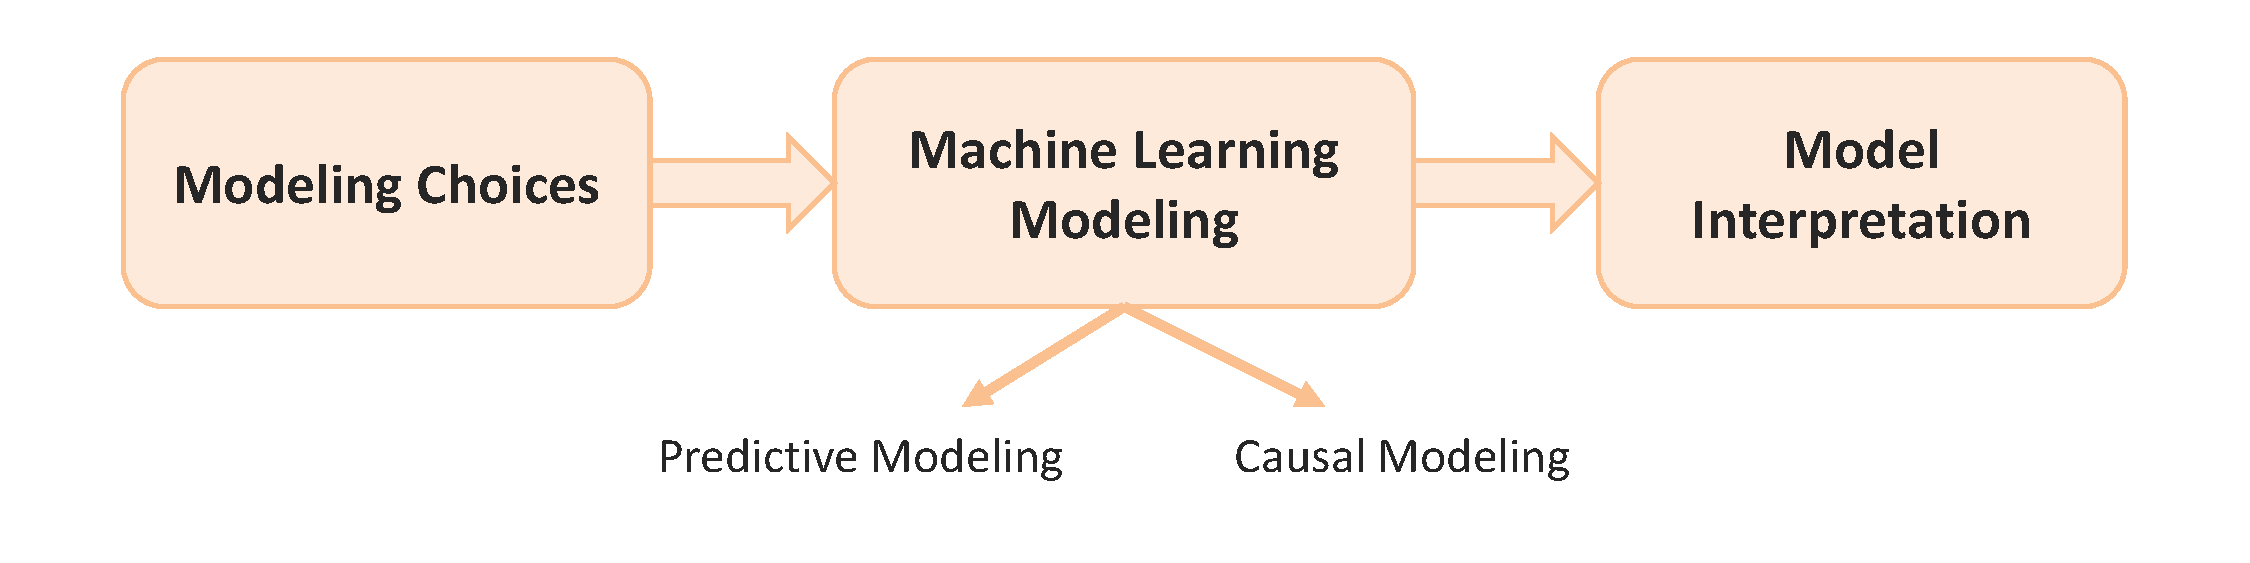
\includegraphics[width=6.5in]{ch1Fig1.pdf}
\caption{Illustration for the typical machine learning modeling pipeline.}
\label{Fig1Ch1}
\end{figure} 

Central to our proposed ML models is the idea of \textit{automation}. In Chapters 4 and 5, we develop methods for making modeling choices in a completely data-driven fashion for both the corss-sectional and longitudinal setups, without the need for manual tuning or expert intervention. Through these automated methods, the ML system is able to craft the model structure by itself so that it best fits the dataset at hand, thereby guarding against na\"ive modeling decisions that may bottleneck the model's predictive accuracy.   \\  
\\ 
\textbf{Stage 2: Machine Learning Modeling}\\
At the core of the modeling pipeline is the actual ML model being used to make predictions. For simple supervised prediction tasks, such as predicting a patient's risk of cardiovascular disease or diabetes based on their age and lifestyle-related variables, one can simply use standard off-the-shelf regression or classification models \cite{weng2017can}. However, many clinical questions cannot be simply reduced to a straightforward prediction problem. As we discuss in detail in Chapter 2, in many cases we would be interested in answering questions such as ``\textit{What is the effect of a given treatment on an individual patient?}'', ``\textit{What is the best treatment option for the patient at hand?}'', or ``\textit{Would this patient have better outcomes had they received a
different medication?}'' For this type of questions, the answer requires inferring the causal effects of interventions, which in turn requires inferring the patient outcomes in counter-factual scenarios that are not observed in the data \cite{morgan2015counterfactuals}. Thus, our core ML models must be able to carry out causal inference tasks and not just predictive inference ones.    

The ML modeling stage should account only for a broad range of clinical questions, but also for different data formats. In the cross-sectional setup, data is simply a static array of variables characterizing the patient state at a given point of time, whereas in the longitudinal setup, data is (irregularly) collected for every patient over time, and each patient may have a different number of observations.  \\ 
\\
\textbf{Stage 3: Model Interpretation}\\
Once the appropriate modeling choices have been made (stage 1), and a model has been trained using the available data (stage 2), we have a functioning ML pipeline in the pragmatic sense --- i.e., we have a model that makes the predictions that we are interested in. However, in almost all clinical setups, this is not enough. An accurate but inscrutable ML model may fail to gain patient and clinician trust. In fact, the conspicuous reluctance of many clinical researchers and epidemiologists to use ML models is often attributed to these models' ``black-box'' nature, which hinders their transparency and interpretability \cite{guidotti2019survey}. 

Because decision support systems based on ML models will be used to inform critical decision-making, clinicians and patients must be able to understand what these models have learned from data and how they makes their predictions. Various regulatory committees have even listed the transparency and intelligibility of prognostic models as a requirement for their deployment \cite{kattan2016american}. The final stage of the ML pipeline thus comprises an interpretation method that enables the users of the ML model to understand its predictions. This stage is inextricable from the preceding stages --- the appropriate kind of model interpretation depends on the ML model being used and format of the data used to train this model. 

\subsection{Outline of the Dissertation}
The rest of this dissertation is organized around the ML pipeline in Figure \ref{Fig1Ch1}. For both the cross-sectional and longitudinal setups, we develop models and algorithms that belong in different stages of the ML pipeline. In what follows, we provide a sneak peek into each of the upcoming chapters, and explain how it relates to the high-level vision in Figure \ref{Fig1Ch1}.  

\label{Sec112}
\subsubsection{Models for Cross-sectional Data} % Technical notation and Figures
Chapters 2, 3 and 4 deal with the 3 stages of the ML pipeline in the cross-sectional setup. In this setup, we examine the relationship between a health outcome $Y$ (e.g., prevalence of a disease, survival outcomes, etc) and patient features $X$ by taking a static ``snapshot of a population'' at a single point of time. (Note that our notion of a ``cross-sectional setup'' corresponds to what is known in the epidemiological literature as \textit{observational studies}, which covers cohort, cross-sectional, and case-control studies.) Chapter 2 starts off with the~core component of the pipeline (stage 2), where we develop a comprehensive framework for ML-based models for causal effect estimation. Chapter 3 proceeds by providing~a~novel symbolic approach for interpreting the predictions of any black-box ML model (stage 3). In Chapter 4, we conclude the ML pipeline for cross-sectional data by developing an algorithm for automating the predictive and causal modeling choices.

\subsubsection{Models for Longitudinal Data}
In Chapter 5, we study the longitudinal setup. In this setup, we are presented sequential data of the form $X_1,.\,.\,.,X_t$ collected for patients who were followed up over an extended period of time. When dealing with longitudinal data, our goal is typically to capture disease trajectories in order to predict patient prognoses in a dynamic fashion and understand the underlying disease mechanisms and dynamics. Unlike in the cross-sectional setup where, in Chapter 5 we do not analyze each stage of the pipeline separately, but rather develop a single comprehensive model for sequential data that executes all stages of the pipeline jointly.     

\subsubsection{Clinical Application}
In Chapter 6, we present a summary of the clinical studies that we conducted based on the ML models developed in earlier chapters. In these studies, we applied our models to cross-sectional data from large-scale cohorts of breast cancer, cardiovascular disease and cystic fibrosis patients, and longitudinal data from the UK cystic fibrosis registry.

\section{Summary of Technical Contributions}
In what follows, we present a brief summary of the technical contributions of each of the upcoming chapters with respect to existing literature.

\label{Sec12}
\subsection*{Chapter 2 Contributions}
In Chapter 2, we consider the problem of using ML to estimate the \textit{causal effect} of a treatment on individual patients on the basis of retrospective, observational data (causal modeling in stage 2 of the pipeline). This problem differs fundamentally from supervised learning since we never observe the treatment effects in the observational data --- we only observe the outcomes of a patient with or without the treatment, but never both. Despite a variety of recently proposed algorithmic solutions to this problem, a principled guideline for building estimators of treatment effects using machine learning algorithms is still lacking. In this chapter, we provide such guidelines by characterizing the fundamental limits of estimating heterogeneous treatment effects, establishing conditions under which these limits can be achieved, and building a practical algorithm for estimating treatment effects based on Gaussian processes. 

\subsection*{Chapter 3 Contributions}
In this Chapter, we tackle stage 3 of the pipeline: understanding the predictions of a general ML model. To this end, we introduce the \textit{symbolic metamodeling} framework --- a general methodology for interpreting predictions by converting ``black-box'' models into ``white-box'' functions that are understandable to human subjects. A symbolic metamodel is a model of a model, i.e., a surrogate model of a trained (machine learning) model expressed through a succinct symbolic expression that comprises familiar mathematical functions and can be subjected to symbolic manipulation. We parameterize metamodels using Meijer $G$-functions --- a class of complex-valued contour integrals that depend on real-valued parameters, and whose solutions reduce to familiar algebraic, analytic and closed-form functions for different parameter settings. This parameterization enables efficient optimization of metamodels via gradient descent, and allows discovering the functional forms learned by a model with minimal a priori assumptions. We show that symbolic metamodeling provides a generalized framework for model interpretation — many common forms of model explanation can be analytically derived from a symbolic metamodel.

\subsection*{Chapter 4 Contributions}
This Chapter addresses stage 1 of the pipeline. We developed an algorithm for automating the design of predictive and causal modeling tailored for clinical prognosis. Our algorithm optimizes ensembles of model configurations efficiently using a novel batched Bayesian optimization (BO) algorithm that learns a low-dimensional decomposition of the models' high-dimensional hyper-parameter space in concurrence with the BO procedure. This is achieved by modeling the models' performances as a black-box function with a Gaussian process prior, and modeling the ``similarities'' between the pipelines' baseline algorithms via a sparse additive kernel with a Dirichlet prior. For causal models, we propose an influence function-based approach to estimate their accuracy.

\subsection*{Chapter 5 Contributions}
Chapter 5 focuses on the longitudinal setup, where we develop a sequential model for predicting patient outcomes and understanding disease dynamics. Existing models provide the patient with pragmatic (supervised) predictions of risk, but do not provide the clinician with intelligible (unsupervised) representations of disease pathology. In this Chapter, we develop the \textit{attentive state-space model}, a deep probabilistic model that learns accurate and interpretable structured representations for disease trajectories. Unlike Markovian state-space models, in which state dynamics are memoryless, our model uses an attention mechanism to create ``memoryful'' dynamics, whereby attention weights determine the dependence of future disease states on past medical history. To learn the model parameters from medical records, we develop an inference algorithm that jointly learns a compiled inference network and the model parameters, leveraging the attentive representation to construct a variational approximation of the posterior state distribution. 


\chapter{Estimating Treatment Effects from Observational Data}

We start off with the core component of the ML pipeline: ML modeling. There is~already~a~wide range of well-established, off-the-shelf predictive models, hence we focus on \textit{causal modeling}. The problem of estimating heterogeneous (individualized) causal effects of a treatment from observational data is central in public health and drug development \cite{foster2011subgroup}. The increasing availability of observational data in these domains has encouraged the development of various machine learning algorithms tailored for inferring treatment effects using observational data (e.g. \cite{li2017matching,wager2017estimation,shalit2016estimating,alaa2017bayesian}). Due to the peculiarity of the treatment effect estimation problem, these algorithms address various modeling aspects that are foreign to standard supervised learning setups; such aspects include ways to handle \textit{sample selection bias} \cite{heckman1977sample}, and ways to model \textit{treated} and \textit{untreated} data points. Despite a variety of recent algorithmic approaches, principled guidelines for model design are lacking. 

In this Chapter, we identify guiding principles for designing practical treatment effect estimation algorithms in the context of Bayesian nonparametric inference, and propose one an algorithm that follows these guidelines. We set these guidelines by characterizing the fundamental limits of estimating treatment effects, and studying the impact of various common modeling choices on the achievability of those limits. In what follows, we provide a brief technical background for the treatment effect estimation problem, along with a summary of our contributions. 

\section{Background and Summary of Contributions}
\label{ch2sec1}
Our analysis hinges on the Rubin-Neyman potential outcomes model \cite{rubin2005causal}. That is, we consider an observational dataset with a population of subjects, where each subject $i$ is endowed with a $d$-dimensional feature $X_i \in \mathcal{X}$. We assume that $\mathcal{X} = [0,1]^d$, but most of our results hold for general compact metric spaces (bounded, closed sets in $\mathbb{R}^d$). A treatment assignment indicator $W_i \in \{0,1\}$ is associated with subject $i$; $W_i = 1$ if the treatment under study was applied to subject $i$, and $W_i = 0$ otherwise. Subject $i$'s responses with and without the treatment (the potential outcomes) are denoted as $Y^{\mbox{\tiny $(1)$}}_i$ and $Y^{\mbox{\tiny $(0)$}}_i$, respectively. Treatments are assigned to subjects according to an underlying policy that depends on the subjects' features, i.e. $W_i \not\!\perp\!\!\!\perp X_i$. This dependence is quantified via the conditional distribution $p(x) = \mathbb{P}(W_i=1|X_i=x)$, also known as the \textit{propensity score} of subject $i$ \cite{rosenbaum1984reducing}. The response $Y^{\mbox{\tiny $(W_i)$}}_i$ is the ``factual outcome" which we observe in the data, whereas $Y^{\mbox{\tiny $(1-W_i)$}}_i$ is the unrealized ``counterfactual outcome" \cite{bottou2013counterfactual}. An observational dataset $\mathcal{D}_n$ comprises $n$ samples of the form: 
\begin{align}
\mathcal{D}_n = \{X_i, W_i, Y^{\mbox{\tiny $(W_i)$}}_i\}_{i=1}^n\,\, 
\label{ch2eq1}
\end{align}
The causal effect of the treatment on subject $i$ with a feature $X_i = x$ is characterized through the \textit{conditional average treatment effect} (CATE) function $T(x)$, which is defined as the expected difference between the two potential outcomes \cite{rubin2005causal}, i.e. 
\begin{align}
T(x) = \mathbb{E}\big[\, Y^{\mbox{\tiny $(1)$}}_i-Y^{\mbox{\tiny $(0)$}}_i\,|\,X_i = x\,\big]
\label{ch2eq2}
\end{align}
Our goal is to identify a set of guiding principles for building estimators of the CATE $T(x)$ using samples from $\mathcal{D}_n$. Throughout this Chapter, we will assume that the density $d\mathbb{P}(X_i,W_i,Y^{\mbox{\tiny $(0)$}}_i,Y^{\mbox{\tiny $(1)$}}_i)$ supports the assumptions of \textit{unconfoundedness} and \textit{overlap}, which are necessary for causal identifiability and consistency. Unconfoundedness requires that  $(Y^{\mbox{\tiny $(0)$}}_i,Y^{\mbox{\tiny $(1)$}}_i) \!\perp\!\!\!\perp W_i\,|\,X_i$, whereas overlap requires that $0 < p(x) < 1$ \cite{rosenbaum1984reducing}. \textbf{Selection bias} occurs in $\mathcal{D}_n$ since the distribution of the treated/control subjects does not match that of the overall population.

In order to come up with principled guidelines for building estimators of $T(x)$, we characterize the fundamental (information-theoretic) limits of estimating the CATE using samples from $\mathcal{D}_n$, and identify the modeling choices that would allow achieving those limits. To this end, in \textbf{Section \ref{ch2sec3}} we tackle the following question: \textbf{what are the fundamental limits of CATE estimation?} We answer this question by deriving the \textit{optimal minimax rate} for estimating $T(x)$ using $\mathcal{D}_n$. Interestingly, it turns out that the optimal rate \textbf{does not} depend on \textbf{selection bias}, but rather on the \textbf{smoothness} and \textbf{sparsity} of the more ``complex" of the functions $\mathbb{E}[\, Y^{\mbox{\tiny $(0)$}}_i\,|\,X_i = x\,]$ and $\mathbb{E}[\, Y^{\mbox{\tiny $(1)$}}_i\,|\,X_i = x\,]$. We focus our analysis on Bayesian nonparametric methods, since they have the appealing properties of being robust to misspecification and are accessible for theoretical analysis. 

Our analysis reveals that the relative importance of the different modeling aspects vary with the sample size. In particular, in the \textbf{large-sample regime}, selection bias does not pose a serious problem, and the model's performance would be mainly determined by its \textbf{structure}, i.e. the way the outcomes $Y^{\mbox{\tiny $(0)$}}_i$ and $Y^{\mbox{\tiny $(1)$}}_i$ are modeled, and the impact of that on variable selection and hyperparameter tuning. On the contrary, selection bias can seriously harm a model's generalization performance in \textbf{small-sample regimes}. A good model should then be carefully designed so that it operates well in both regimes by possessing the right \textbf{model structure} that would allow learning at a fast rate, and the right \textbf{model selection} (hyperparameter optimization) scheme that would account for selection bias. 
   
In Section \ref{ch2sec4}, we build a practical CATE estimation algorithm guided by the results of the analyses in Section \ref{ch2sec3}. We model the outcomes $Y^{\mbox{\tiny $(0)$}}_i$ and $Y^{\mbox{\tiny $(1)$}}_i$ using a Gaussian process with a \textit{non-stationary} kernel that captures the different relevant variables and different levels of smoothness of the functions $\mathbb{E}[\, Y^{\mbox{\tiny $(0)$}}_i\,|\,X_i = x\,]$ and $\mathbb{E}[\, Y^{\mbox{\tiny $(1)$}}_i\,|\,X_i = x\,]$. We prove that this model structure can achieve the optimal rate of CATE estimation when tuned with the right hyperparameters. We also propose a \textit{doubly-robust} hyperparameter optimization scheme that accounts for selection bias in small-sample regimes, without hindering the model's minimax-optimality in the large sample limit. We show that our algorithm outperforms state-of-the-art methods using a well-known semi-synthetic simulation setup.

\section{Related Work}
Very few works have attempted to characterize the limits of CATE estimation, or study the impact of different modeling choices on the CATE estimation performance in a principled manner. \cite{alaa2017bayesian2} characterized the asymptotic ``information rates" for different CATE estimators, but provided no clear guidelines on practical model design or an analysis of the impact of sample selection bias. The study in \cite{kunzel2017meta} was rather empirical in nature, comparing the performance of different regression structures for the potential outcomes while ignoring selection bias. A similar study, but focusing only on random forest models, was conducted in \cite{lu2017estimating}.   

Most of the previous works have been algorithmic in nature, focusing mainly on devising algorithms that correct for selection bias (e.g. \cite{johansson2016learning,jjschaar,wager2017estimation,li2017matching}). Some of these works cast the selection bias problem as a problem of \textit{covariate shift} \cite{sugiyama2007covariate}, and use techniques from \textit{representation learning} to learn feature maps that balance the biased data (e.g. \cite{li2017matching,shalit2016estimating,johansson2016learning}). However, those works report much bigger improvements in CATE estimation when changing their model structure (e.g. architecture of a neural network), as compared to the gains attained by only accounting for bias (see the comparisons between the TARnet and BNN models in \cite{shalit2016estimating}). Similar observations are reported in \cite{alaa2017bayesian,Onur1}, where the selection of the model structure seemed to influence the achieved CATE estimation performance even when selection bias is not accounted for. However, none of these works offer a discussion on whether selection bias is actually the main challenge in CATE estimation, or whether the outcomes' model structure may have a bigger influence on performance.

In contrast to the works above, in this Chapter we do not attempt to develop a model by presupposing that particular modeling aspects are of greater importance than others, but rather provides a framework for understanding the limits on the achievable performance, and how different modeling aspects influence a model's chance of achieving those limits. We use our analyses to both reflect on the modeling choices made in the works above, and also devise a novel, principled CATE estimation algorithms that achieves the fundamental performance limits.  

\section{Estimating CATE: Problem Setup} 
\label{ch2sec3}
\subsection{Potential Outcomes and Propensity Score}
\label{pO22}
We consider the following \textit{random design} regression model for the potential outcomes:
\begin{equation}
Y^{\mbox{\tiny $(w)$}}_i = f_{w}(X_i) + \varepsilon_{i,w},\, w \in \{0,1\},  
\label{ch2eq3}
\end{equation}
where $\varepsilon_{i,w} \sim \mathcal{N}(0,\sigma^2_{w})$ is a Gaussian noise variable. It follows from (\ref{ch2eq2}) that the CATE is $T(x) = f_{1}(x)-f_{0}(x)$. The \textit{response surfaces} $f_{1}(x)$ and $f_{0}(x)$ correspond to the subjects' responses with and without the treatment. We assume that $f_{w}(.): \mathcal{X} \rightarrow \mathbb{R}$, $w \in \{0,1\}$, is a totally bounded function that lives in a space of ``smooth" or ``regular" functions, with an unknown smoothness parameter $\alpha_{w}$. We use H\"older balls for concreteness, although our results extend to other function spaces. A function $f_{w}(.)$ lies in the H\"older ball $H^{\alpha_{w}}$, with a H\"older exponent $\alpha_{w} > 0$, if and only if it is bounded in sup-norm by a constant $C > 0$, all its partial derivatives up to order $\lfloor \alpha_{w} \rfloor$ exist, and all its partial derivatives of order $\lfloor \alpha_{w} \rfloor$ are Lipschitz with exponent $(\alpha_{w}-\lfloor \alpha_{w} \rfloor)$ and constant $C$. The H\"older exponents quantify the complexities of $f_0$ and $f_1$, and hence the hardness of estimating $T(x)$ would depend on $\alpha_{0}$ and $\alpha_{1}$. 

\subsection{Bayesian Nonparametric Inference}
Nonparametric inference is immune to misspecification of the outcomes' and propensity models \cite{kennedy2018nonparametric}, and hence we focus on Bayesian nonparametric methods for inferring $T(.)$ on the basis of $\mathcal{D}_n$. Bayesian inference entails specifying a prior distribution $\Pi$ over $f_1(.)$ and $f_0(.)$, i.e.
\begin{equation}
f_0, f_1 \sim \Pi(\bar{\varphi}_{\beta_0}, \bar{\varphi}_{\beta_1}),
\label{ch2eq4}
\end{equation}
where $\bar{\varphi}_{\beta_w} = \{\varphi^k_{\beta_w}\}_{k=1}^\infty, w \in \{0,1\},$ are complete orthonormal bases (indexed by a parameter $\beta_w > 0$) with respect to Lebesgue measure in $\mathcal{X}$, $f_w = \sum_k \bar{f}^k_w \cdot \varphi^k_{\beta_w},$ and $\bar{f}^k_w = \langle f_w, \varphi^k_{\beta_w}\rangle$. Thus, for given bases $\bar{\varphi}_{\beta_0}$ and $\bar{\varphi}_{\beta_1}$, $\Pi$ places a probability distribution on the projections $\{\bar{f}^k_w\}_k$. Potential choices for the basis $\bar{\varphi}_{\beta_w}$ that would give rise to implementable Bayesian inference algorithms include regular wavelet basis \cite{zhang1997using}, radial basis for a reproducing kernel Hilbert space (RKHS) \cite{van2008reproducing}, etc. In general, $\beta_w$ would determine the smoothness of the function space spanned by $\bar{\varphi}_{\beta_w}$. 

\subsection{Towards Principled CATE Estimation} 
To evaluate the predictive accuracy of the Bayesian inference procedure, we analyze the ``frequentist" loss of point estimators $\hat{T}(x)$ induced by the Bayesian posterior $d\Pi_n(T(x)\,|\,\mathcal{D}_n)$, assuming that $\mathcal{D}_n$ is generated based on fixed, \textit{true} response surfaces $f_{1}(x)$ and $f_{0}(x)$. (This type of analysis is sometimes referred to as the ``Frequentist-Bayes" analysis \cite{sniekers2015adaptive}.) In particular, we quantify the performance of a point estimator $\hat{T}(x) = \delta(d\Pi_n(T(x)\,|\,\mathcal{D}_n))$ by its squared-$L^2(\mathbb{P})$ error, which was dubbed the \textit{precision of estimating heterogeneous effects} \textbf{(PEHE)} in \cite{hill2011bayesian}, and is formally defined as:
\begin{align}
\mathbold{\psi}(\hat{T}) &\triangleq \mathbb{E}\,\|\,\hat{T} - T\,\|^2_{\mbox{\tiny $L^2(\mathbb{P})$}}, 
\label{ch2eq5}
\end{align} 
where $L^2(\mathbb{P})$ is the $L^2$ norm with respect to $\mathbb{P}(X)$, i.e. $\|f(x)\|^2_{\mbox{\tiny $L^2(\mathbb{P})$}} = \int f^2(x)\, d\mathbb{P}(X=x)$.

The ``fundamental problem of causal inference" is that for every subject $i$ in $\mathcal{D}_n$, we only observe the \textbf{factual} outcome $Y^{\mbox{\tiny $(W_i)$}}_i$, whereas the \textbf{counterfactual} $Y^{\mbox{\tiny $(1-W_i)$}}_i$ remains unknown, which renders empirical evaluation of the PEHE in (\ref{ch2eq5}) impossible. Moreover, $\mathcal{D}_n$ would generally exhibit sample \textbf{selection bias} \cite{heckman1977sample}, because the treatment assignment mechanism (decided by $p(x)$) creates a discrepancy between the feature distributions of the treated/control population and the overall population. Thus, standard \textbf{supervised learning} approaches based on empirical risk minimization cannot be used to learn a generalizable model for the CATE from samples in $\mathcal{D}_n$. This gives rise to the following fundamental modeling questions that are peculiar to CATE estimation:
\begin{itemize} % HOW DO THEY RELATE TO THE PRIOR
\item \textbf{[Q1]:} How should the treatment assignment $W_i$ be incorporated into the learning model? % structure of the prior
\item \textbf{[Q2]:} How should selection bias be handled? % how to adapt the prior
\end{itemize}

Adequate answers to \textbf{[Q1]} and \textbf{[Q2]} would provide guidelines for selecting the prior $\Pi(\bar{\varphi}_{\beta_0}, \bar{\varphi}_{\beta_1})$. Addressing the modeling questions above requires a profound understanding of the \textbf{fundamental limits} of CATE estimation, in addition to an understanding of the impact of different modeling choices on the \textbf{achievability} of such limits. The next Sections provide principled answers to \textbf{[Q1]} and \textbf{[Q2]} by addressing the following, more fundamental questions:
\begin{itemize}
\item \textbf{\underline{Section \ref{ch1sec3}}: What are the \textit{limits} on the performance achieved by \textit{any} CATE estimator?}
\item \textbf{\underline{Section \ref{ch2sec4}}: How can we build \textit{practical algorithms} that can achieve these limits?}
\end{itemize}

\section{Fundamental Limits of CATE Estimation} %1 Theorem, 2- Holder codewords and hamming 3- remarks
\label{ch1sec3} 
In this Section, we establish an information-theoretic limit on the performance of \textit{any} CATE estimator. In what follows, we use the standard Bachmann-Landau order notation, and write $a \vee b = \max\{a,b\},$ $a \wedge b = \min\{a,b\}$. The notation $a \lesssim b$ means that $a \leq C b$ for a universal constant $C$, and $\asymp$ denotes asymptotic equivalence. 

\subsection{Optimal Minimax Rates}
\label{BMS2}
The ``hardness" of a nonparametric estimation problem is typically characterized by its \textit{minimax} risk \cite{stone1982optimal}, i.e. the minimum worst case risk achieved by \textit{any} estimator when the estimand is known to live in a given function space \cite{yang2015minimax}. In the following Theorem, we establish the optimal minimax rate for the PEHE risk in terms of the complexity of the response surfaces $f_0$ and $f_1$.\\ 
\\
\textbf{Theorem~1.} \textit{Suppose that $\mathcal{X} = [0,1]^d$, and that $f_w$ depends on a subset of $d_w$ features with $d_w \leq \min\{n,d\}$ for $w \in \{0,1\}$. If $f_0 \in H^{\alpha_0}$ and $f_1 \in H^{\alpha_1}$, then the optimal minimax rate is:} 
\begin{align}
\inf_{\hat{T}} \sup_{f_0,f_1} \mathbold{\psi}(\hat{T}) \,\asymp\, \underbrace{n^{-\left(1+\frac{1}{2}\left(\frac{d_0}{\alpha_0}\vee \frac{d_1}{\alpha_1}\right)\right)^{-1}}}_{\textbf{CATE\,\, estimation}} \vee \underbrace{\log \mbox{\footnotesize$\left(\frac{d^{d_0+d_1}}{d_0^{d_0}\, d_1^{d_1}}\right)^{\frac{1}{n}}$}.}_{\textbf{Variable\,\, selection}}\nonumber
\end{align} 
\textit{The above holds for any $p(.) \in H^{\alpha_p}$, $\alpha_p > 0$.} \,\,\, $\mathbf{\Box}$ \\

In Theorem 1, the supremum is taken over $\alpha_w$-H\"older balls ($w \in \{0,1\}$), whereas the infimum is taken over all possible Bayesian estimators. The~minimax~rate~in~Theorem~1 corresponds to the \textbf{fastest rate} by which \textbf{any} (Bayesian) estimator $\hat{T}(.)$ can approximate the CATE function $T(.)$. The proof of Theorem 1 (provided in the supplement) uses information-theoretic techniques based on Fano's method to derive algorithm-independent estimation rates \cite{yang1999information}. In the following set of remarks, we revisit \textbf{[Q1]} and \textbf{[Q2]} in the light of the results of Theorem 1.\\ 
\\ 
\textbf{How can Theorem 1 help us address \mbox{\footnotesize \textbf{[Q1]}} and \mbox{\footnotesize \textbf{[Q2]}}?}\\
\\
$\triangleright$ \textbf{Remark 1 (Smoothness and sparsity)}

Theorem 1 says that estimating CATE is as hard as nonparametric regression for functions with additive sparsity \cite{raskutti2009lower,yang2015minimax}. The minimax rate in Theorem 1 decomposes into a term reflecting the complexity of CATE estimation under correct variable selection for $f_0$ and $f_1$, and a term reflecting the complexity of variable selection. Variable selection complexity remains small as long as $\log(d) = \Theta(n^\zeta),$ for some $\zeta \in (0,1)$, and approaches the parametric rates as $\zeta \to 0$. The minimax rate will generally be dominated by the complexity of CATE estimation, and will approach the parametric rates only for very smooth response surfaces with small number of relevant dimensions, i.e. $\frac{d_0}{\alpha_0} \vee \frac{d_1}{\alpha_1} \to 0$.    

The main takeaway from Theorem 1 is that the CATE learning rate is determined by the more ``complex" of the surfaces $f_0$ and $f_1$, where complexity is quantified by the sparsity-to-smoothness ratio $d_w/\alpha_w$ for $w \in \{0,1\}$. Thus, a model would achieve the optimal CATE learning rate only if it selects the correct relevant variables for $f_0$ and $f_1$, and tunes its ``hyperparameters" (i.e. smoothness of the prior) to cope with a complexity of $\frac{d_0}{\alpha_0} \vee \frac{d_1}{\alpha_1}$. When $\frac{d_0}{\alpha_0}$ and $\frac{d_1}{\alpha_1}$ are very different (e.g. $f_0$ and $f_1$ have different relevant features), rate-optimal estimation is possible only if the model incorporates such differences in $\Pi(\bar{\varphi}_{\beta_0},\bar{\varphi}_{\beta_1})$. % bases

The discussion above \textbf{provides a concrete answer to \mbox{\footnotesize \textbf{[Q1]}}:} the treatment assignment variable $w$ should be incorporated into the model in such a way that it \textbf{encodes the different relevant dimensions and smoothness levels of $\boldsymbol{f_0}$ and $\boldsymbol{f_1}$ in the bases $\boldsymbol{\bar{\varphi}_{\beta_0}}$ and $\boldsymbol{\bar{\varphi}_{\beta_1}}$}. (The simplest way to achieve this is to use two separate models for $f_0$ and $f_1$.) This is not fulfilled by many of the previous models that built a single regression function of the from $f: \mathcal{X} \times \{0,1\} \to \mathbb{R}$, and estimated the CATE as $\hat{T}(x) = f(x,1) - f(x,0)$ \cite{hill2011bayesian,johansson2016learning,powers2017some}. This is because such models enforced the smoothness of the prior along all features to be the same for $w = 0$ and $w = 1$.\\ 
\\    
$\triangleright$ \textbf{Remark 2 (Selection bias)} 

Theorem 1 gives a rather surprising answer to \textbf{[Q2]}: the \textbf{optimal learning rate} is \textbf{oblivious to selection bias}. Such a finding is consistent with previous results on nonparametric kernel density estimation under selection bias \cite{borrajo2017bandwidth}, and parametric Bayesian inference under \textit{covariate shift} \cite{shimodaira2000improving,sugiyama2007mixture}. It shows that many of the recent works have missed the target; the works in \cite{johansson2016learning,shalit2016estimating,alaa2017bayesian} cast the problem of CATE estimation as one of \textbf{covariate shift} that results from selection bias. However, Theorem 1 says that selection bias is not a problem when we have a sufficiently large amount of data. This is because selection bias is inherently a misspecification problem, and hence its impact on nonparametric inference is washed away in large-sample regimes. 

Remarks 1 and 2 posit an explanation for various recurrent (empirical) findings reported in previous literature. For instance, \cite{hahn2017bayesian} found that separate modeling of $f_0$ and $f_1$ via Bayesian additive regression trees (BART) outperforms the well-known single-surface BART model developed in \cite{hill2011bayesian}. Similar findings were reported for models based on Gaussian processes \cite{alaa2017bayesian}, and models based on deep neural networks \cite{shalit2016estimating}. All such findings can be explained in the light of Remark 1. On the other hand, Remark 2 may provide an explanation as to why the ``TARnet" model in \cite{shalit2016estimating}, which models $f_0$ and $f_1$ using separate neural networks and does not account for selection bias, outperformed the ``BNN" model in \cite{johansson2016learning}, which regularizes for selection bias but fits a single-output network for $f_0$ and $f_1$. 

\subsection{Backing off from ``Asymptopia"} 
\label{backasymp}
Theorem 1 shows that selection bias does not hinder the optimal minimax rates, and that it is only the structural properties of the prior $\Pi(\bar{\varphi}_{\beta_0},\bar{\varphi}_{\beta_1})$ that determine a model's rate of learning. But does the achieved learning rate suffice as a sole criterion for addressing the modeling questions \textbf{[Q1]} and \textbf{[Q2]}? The answer is ``yes" only if $\mathcal{D}_n$ comes from a large observational dataset, in which case the learning rate suffices as a descriptor for the large-sample performance. However, if $\mathcal{D}_n$ is small, which is typical in post-hoc analyses of clinical trials \cite{foster2011subgroup}, then one should make the design choices that would optimize the small-sample performance. In order to give a complete picture of the performance in large and small-sample regimes, we derive the following bound on the PEHE:
\begin{align}
\mathbold{\psi}(\hat{T}) &\leq \bar{C}\cdot \exp(D_2(Q_0\,\|\,Q))\cdot\|f_0-\hat{f}_0\|^2_{L^2(\mathbb{P}_0)} + \bar{C}\cdot \exp(\underbrace{D_2(Q_1\,\|\,Q)}_{\substack{\textbf{Reyni}\\ \textbf{Divergence}}})\cdot\underbrace{\|f_1-\hat{f}_1\|^2_{L^2(\mathbb{P}_1)}}_{\substack{\textbf{Supervised}\\ \textbf{learning\,\,loss}}},
\label{ch2eq7} 
\end{align}	
for some $\bar{C} > 0$, where $L^2(\mathbb{P}_w)$, for $w \in \{0,1\},$ is the $L^2$ norm with respect to $d\mathbb{P}(X=x\,|\,W=w)$, $Q = d\mathbb{P}(X=x)$, $Q_w = d\mathbb{P}(X=x\,|\,W=w)$, and $D_{m}(p\,\|\,q)$ is the $m^{th}$ order R\'eyni divergence. The bound in (\ref{ch2eq7}) holds for all $n > 0$, and is tight (refer to the Appendix); it shows that the PEHE is a weighted linear combination of the mean squared losses for the two underlying supervised problems of learning $f_0$ and $f_1$ with \textbf{no covariate shift}, where the weights are determined by the extent of the mismatch between the distributions of the treated and control populations, quantified by the R\'eyni divergence measure. If $\mathcal{D}_n$ is a dataset obtained from a randomized controlled trial ($Q=Q_0=Q_1$), then we have $D_2(Q_0\,\|\,Q)=D_2(Q_1\,\|\,Q) = 0$, and the bound boils down to a sum of two supervised learning losses, i.e. $\mathbold{\psi}(\hat{T}) \leq \bar{C}\cdot\|f_0-\hat{f}_0\|^2_{L^2(\mathbb{P})} + \bar{C}\cdot\|f_1-\hat{f}_1\|^2_{L^2(\mathbb{P})}$.

Since the minimax rate for standard nonparametric regression is $\|f_w-\hat{f}_w\|^2_{2} \asymp C_w \cdot n^{\frac{-2\alpha_w}{2\alpha_w + d_w}}$ \cite{stone1982optimal}, when $d_0/\alpha_0 >> d_1/\alpha_1$, the first-order Taylor approximation for the logarithm of the PEHE in (\ref{ch2eq7}) is given by:
\begin{align}
\log(\mathbold{\psi}(\hat{T})) \approx \, \underbrace{D_2(Q_0\|Q)}_{\substack{\textbf{Selection}\\ \textbf{bias}}} + \underbrace{\log(C_0)}_{\substack{\textbf{Bias}\\ \textbf{correction}}} - \underbrace{\frac{2\alpha_0}{2\alpha_0 + d_0}}_{\substack{\textbf{Learning\, rate}}}\log(n) +\, O\left(n^{\frac{-2\alpha_1}{2\alpha_1 + d_1}+\frac{2\alpha_0}{2\alpha_0 + d_0}}\right).
\label{ch2eq8}
\end{align}
That is, when viewed on a $\log$-$\log$ scale, the behavior of the PEHE versus the number of samples can be described as follows. $\log(\mbox{PEHE})$ is a linear function of $\log(n)$. Selection bias adds a constant offset to $\log(\mbox{PEHE})$, but does not affect its slope, which harms the performance only in the small-sample regime. In the large-sample regime, the slope of $\log(\mbox{PEHE})$, which depends solely on the smoothness and sparsity of the response surfaces, dominates the performance, and selection bias becomes less of a problem. Figure \ref{ch2fig1} depicts the PEHE in (\ref{ch2eq8}) on a $\log$-$\log$ scale.
		
\begin{figure}[t]
\centering
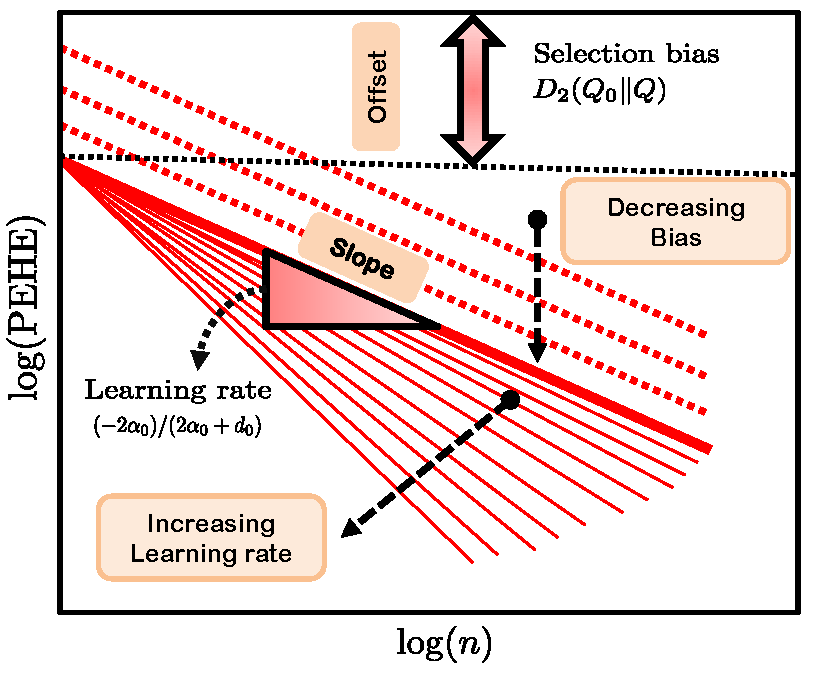
\includegraphics[width=3.5in]{logpehe.pdf}
\caption{The PEHE in (\ref{ch2eq8}) plotted on a $\log$-$\log$ scale.}
\label{ch2fig1}
\end{figure}
 
\section{CATE Estimation using Non-Stationary Gaussian Process Regression}
\label{ch2sec4}
In this Section, we build on the analyses conducted in Section \ref{ch1sec3} to design a practical algorithm for CATE estimation. 

\subsection{Non-Stationary Gaussian Process Priors} 
\label{ch2sec41} 
We specify the prior $\Pi(\bar{\varphi}_{\beta_0},\bar{\varphi}_{\beta_1})$ as a Gaussian process (GP) over $g: \mathcal{X} \times \{0,1\} \to \mathbb{R}$, with a kernel $\boldsymbol{K}_{\beta}$, and a hyperparameter set $\beta$ as follows:
\begin{align}  
g \sim \mathcal{GP}\left(0,\boldsymbol{K}_{\beta}(z,z^{\prime})\right),
\label{ch2eq9}
\end{align}
where $z = (x,w) \in \mathcal{X} \times \{0,1\},$ and $f_w(x) = g(x,w)$. The kernel $\boldsymbol{K}_{\beta}$ specifies the bases $\bar{\varphi}_{\beta_0}$ and $\bar{\varphi}_{\beta_1}$ through its induced canonical feature map $\boldsymbol{K}_{\beta}(.,z)$ \cite{rasmussen2006gaussian,alvarez2012kernels}. As pointed out in \textbf{Remark 1}, the treatment assignment variable $w$ should encode the different relevant dimensions and smoothness levels of $f_0$ and $f_1$. Thus, we model $\boldsymbol{K}_{\beta}$ as a \textit{non-stationary} kernel that depends on $w$ as follows:      
\begin{align}  
\boldsymbol{K}_{\beta}(z,z^{\prime}) &= \boldsymbol{\Gamma}(w,w^{\prime}) \cdot \boldsymbol{k}_{\beta}^{T}(x,x^{\prime}), \nonumber \\
\boldsymbol{k}_{\beta}(x,x^{\prime}) &= \left[k_{\beta_0}(x,x^{\prime}),k_{\beta_1}(x,x^{\prime}),k_{\beta_0}(x,x^{\prime}) + k_{\beta_1}(x,x^{\prime})\right], \nonumber \\
\boldsymbol{\Gamma}(w,w^{\prime}) &= \left[\Gamma_{0}(w,w^{\prime}),\Gamma_{1}(w,w^{\prime}),1-\Gamma_{0}(w,w^{\prime})-\Gamma_{1}(w,w^{\prime})\right], \nonumber
\end{align}
where $\Gamma_{0}(w,w^{\prime}) = (1-w)(1-w^{\prime})$, $\Gamma_{1}(w,w^{\prime}) = w\cdot w^{\prime}$, and $k_{\beta_w}(x,x^{\prime})$ is a Mat\'ern kernel with a length-scale parameter $\beta_w$, for $w \in \{0,1\}$. The kernel defined above ensures that any covariance matrix induced by points in $\mathcal{X}\times\{0,1\}$ is positive definite. Variable selection is implemented by using the \textit{automatic relevance determination} version of the Mat\'ern kernel \cite{rasmussen2006gaussian}. The non-stationarity of $\boldsymbol{K}_{\beta}$ allows setting \textbf{different} length-scales and relevant variables for the marginal priors on $f_0$ and $f_1$ while sharing data between the two surfaces, i.e.
\begin{align}  
\boldsymbol{K}_{\beta}((x,w),(x^{\prime},w)) &= k_{\beta_w}(x,x^{\prime}),\,\, w \in \{0,1\}, \nonumber \\
\boldsymbol{K}_{\beta}((x,w),(x^{\prime},w^{\prime})) &= k_{\beta_0}(x,x^{\prime}) + k_{\beta_1}(x,x^{\prime}),\, w \neq w^{\prime}.
\label{ch2eq10}
\end{align}

That is, all draws from the prior give Mat\'ern sample paths with different smoothness levels ($\beta_0$ and $\beta_1$) for $f_0$ and $f_1$, respectively, and the correlations between the paths are captured via the kernel mixture $k_{\beta_0}(x,x^{\prime}) + k_{\beta_1}(x,x^{\prime})$. Note that draws from a Mat\'ern prior with length-scale $\beta$ are almost surely $\bar{\beta}$-H\"older for all $\bar{\beta} \leq \beta$ \cite{vaart2011information}. Thus, $\mathcal{GP}(0,\boldsymbol{K}_{\beta})$ specifies a $\beta_w$-H\"older ball as an a priori regularity class for response surface $f_w,\, w \in \{0,1\}$. 

In the following Theorem, we show that point estimators induced by the prior $\mathcal{GP}(0,\boldsymbol{K}_{\beta})$ can achieve the optimal minimax rate in Theorem 1.\\
\\
\textbf{Theorem~2.} \textit{Suppose that the $d_w$ relevant features for $f_w$ are known a priori for $w \in \{0,1\}$. If $f_0 \in H^{\alpha_0}$, $f_1 \in H^{\alpha_1}$, $\Pi = \mathcal{GP}(0,\boldsymbol{K}_{\beta})$, and $\hat{T} = \mathbb{E}_{\Pi}[\,T\,|\,\mathcal{D}_n\,]$, then we have that} 
\begin{align}
\mathbold{\psi}(\hat{T}) \,\lesssim\, n^{-\frac{2(\alpha_0 \wedge \beta_0)}{2\beta_0 + d_0}} \vee n^{-\frac{2(\alpha_1 \wedge \beta_1)}{2\beta_1 + d_1}}  
\nonumber
\end{align} 
\textit{whenever $\min\{\alpha_0, \alpha_1, \beta_0, \beta_1\} \geq d/2$.} \,\,\, $\mathbf{\Box}$

Note that posterior consistency holds for all combinations of $(\alpha_0, \alpha_1, \beta_0, \beta_1)$ since the support of the Mat\'ern prior is the space of bounded continuous functions\footnote{This is because the RKHS associated with the prior lies dense in the space of bounded continuous functions \cite{van2008rates,van2008reproducing}.}. The bound in Theorem 2 can be shown to be tight using the results in \cite{castillo2008}. Theorem 2 says that the posterior induced by the prior $\mathcal{GP}(0,\boldsymbol{K}_{\beta})$ contracts around the true CATE function at the optimal rate given in Theorem 1 provided that the following \textbf{matching condition} is met:   
\begin{align}
\beta_v \,\,&= \alpha_v \nonumber \\
\alpha_{v}\frac{d_{1-v}}{d_v} \,\,&\leq \beta_{1-v} \leq \alpha_{1-v} + \frac{\alpha_{1-v}\cdot d_{v}}{2\alpha_{v}}-\frac{d_{1-v}}{2},
\label{ch2eq11}
\end{align}
where $v = 1$ if $d_1/\alpha_1 > d_0/\alpha_0$, and $v = 0$ otherwise. The condition in (\ref{ch2eq11}) implies that achieving the optimal rate (steepest slope in Figure \ref{ch2fig1}) via the non-stationary GP prior in Section \ref{ch2sec41} is only a matter of hyperparameter tuning: the smoothness of the prior needs to match the smoothness of the ``more complex" of the two response surfaces. Note that Theorem 2 implies that we do not need to handle selection bias in order to achieve the optimal rate, which is consistent with the earlier discussion in \textbf{Remark 2}. 
%%%%%%%%%%%%%%%%%%%%%%%%%%%%%%%%%%%%%%%%%%%%%%%%%%%%%%%%%%%%%%%%%%%%%%

\subsection{Doubly-Robust Hyperparameters}
\label{modsec}
Theorem 2 says that the optimal minimax rate for CATE estimation can be achieved by satisfying the smoothness matching condition in (\ref{ch2eq11}). However, in practice, the smoothness levels of the true response functions are unknown and need to be learned from the data. Moreover, since selection bias is impactful in small-sample regimes, ignoring it may lead to a poor generalization performance when the size of $\mathcal{D}_n$ is small. In this Section, we propose a hyperparameter optimization algorithm that accounts for selection bias while ensuring minimax-optimality in the large-sample limit.

Previous works tend to adjust for selection bias ``mechanically" using variants of importance sampling approaches based on inverse-propensity-weighting (IPW) \cite{sugiyama2007covariate,shimodaira2000improving}, and kernel mean matching \cite{huang2007correcting}, or by learning a ``balanced representation" of treated and control populations \cite{li2017matching}. We do not attempt to explicitly adjust for selection bias using ad-hoc approaches, and rather seek the ``informationally optimal" estimator of the PEHE. That is, we seek the \textbf{most efficient} (unbiased) estimator $\hat{\psi}^{*}(\hat{T})$ of $\psi(\hat{T})$, which satisfies an analog of the Cram\'er-Rao bound (information-inequality) in parametric estimation, i.e. $\mbox{Var}[\hat{\psi}^{*}(\hat{T})] \leq \mbox{Var}[\hat{\psi}(\hat{T})]$, for any estimator $\hat{\psi}(\hat{T})$. 

Classical Cram\'er-Rao bounds do not apply to estimators of the form $\hat{\psi}^{*}(\hat{T})$, since such estimators are functionals of nonparametric objects. There are, however, analogous information inequalities for nonparametric estimation, including Bhattacharyya's variance bound \cite{bhattacharyya1946some}, and its generalization due to Bickel \cite{bickel1998efficient}. We proceed by realizing that the PEHE $\psi(\hat{T})$ is simply a functional that belongs to the \textit{doubly-robust} class of functionals analyzed by Robins in \cite{robins2008higher}. Thus, one can construct the ``most" efficient estimator of $\psi(\hat{T})$ using the most \textit{efficient influence function} of $\psi(\hat{T})$ as follows \cite{robins2008higher,robins2004optimal}:  
\begin{align}
\hat{\psi}^{*}(\hat{T}) = \sum^n_{i=1} \left(\frac{Y^{\mbox{\tiny $(W_i)$}}_i-(W_i-p(X_i))\cdot\hat{T}(X_i)}{p(X_i)\cdot(1-p(X_i))}\right)^2. \nonumber 
\end{align}
The derivation of the estimator above can be found in Theorem 9 in \cite{robins2004optimal} and Section 5 in \cite{robins2008higher}. When the propensity function $p(.)$ is known, this estimator approximate the PEHE at its optimal minimax rate. We estimate $p(.)$ via standard kernel density estimation methods. It can be easily shown using the results in \cite{dudoit2005asymptotics} that when using the estimator above to tune the GP hyperparameters via cross-validation, then the learned length-scale parameters will satisfy the matching condition for minimax optimality. 

\begin{figure*}[t]
\centering
\begin{subfigure}{.33\textwidth}
  \centering
  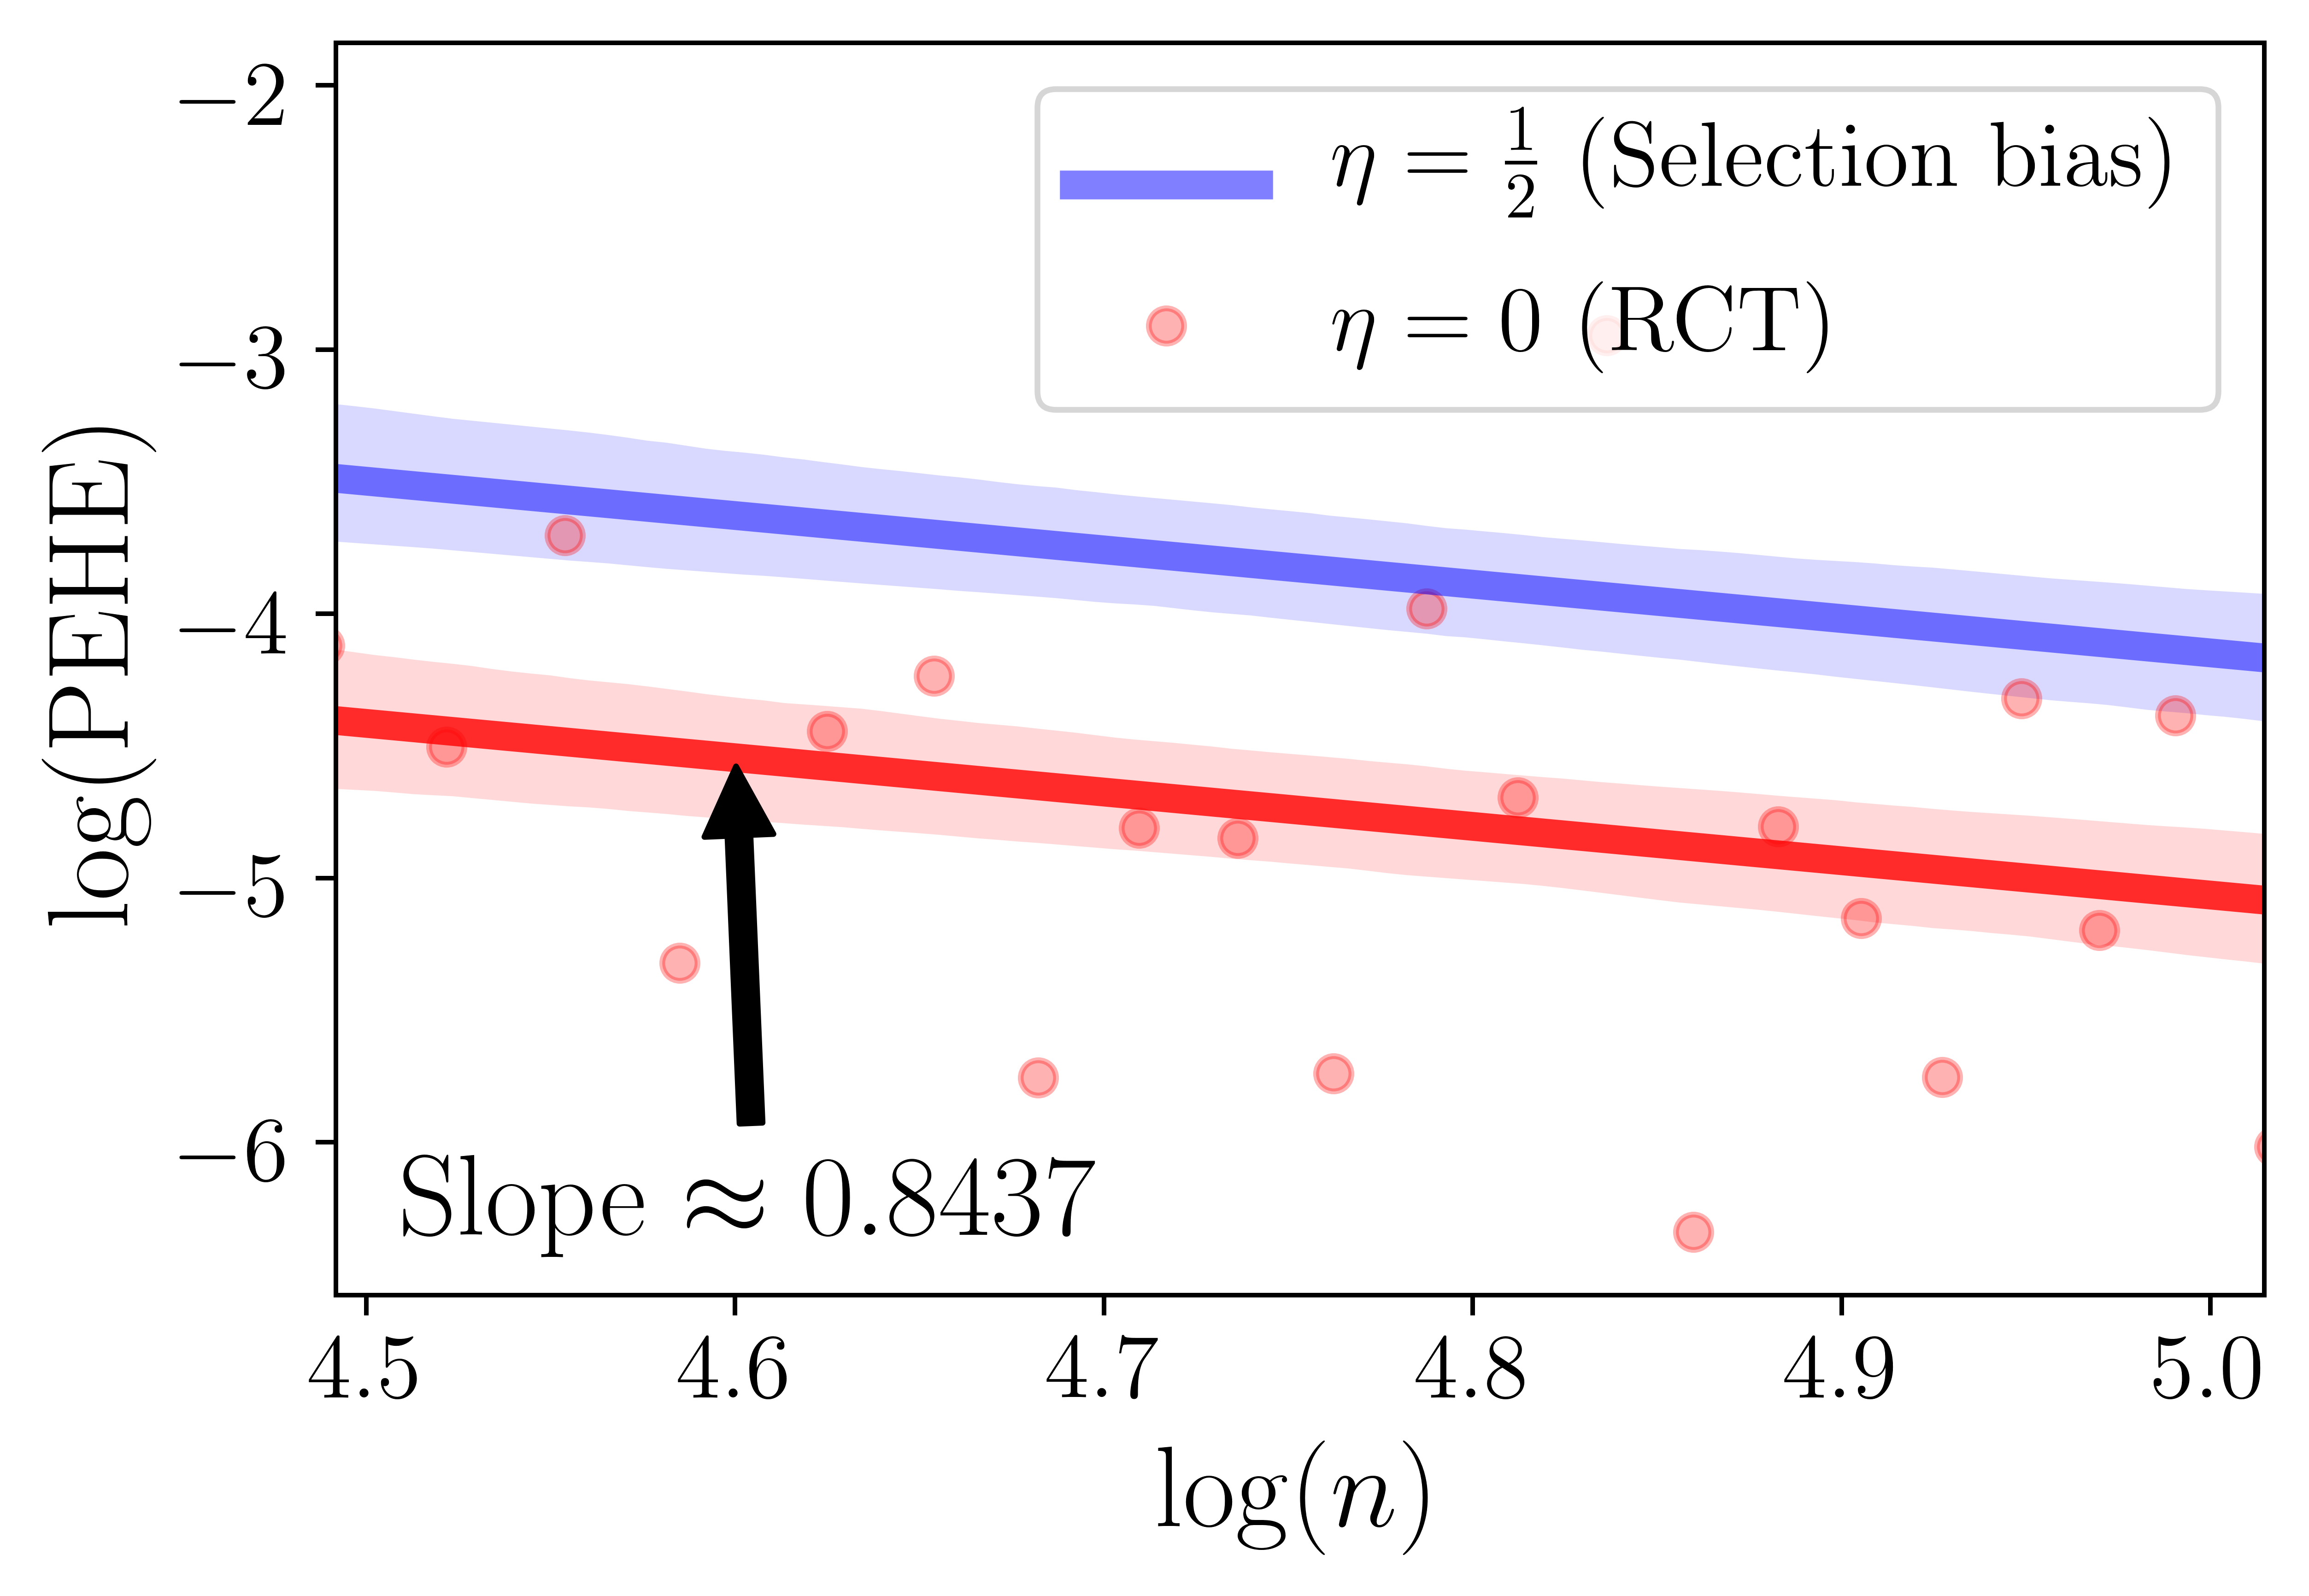
\includegraphics[width=0.9\linewidth]{ch2Fig2.png}
  \caption{\footnotesize Impact of selection bias.}
  \label{Ahmed1}
\end{subfigure}%
\begin{subfigure}{.33\textwidth}
  \centering
  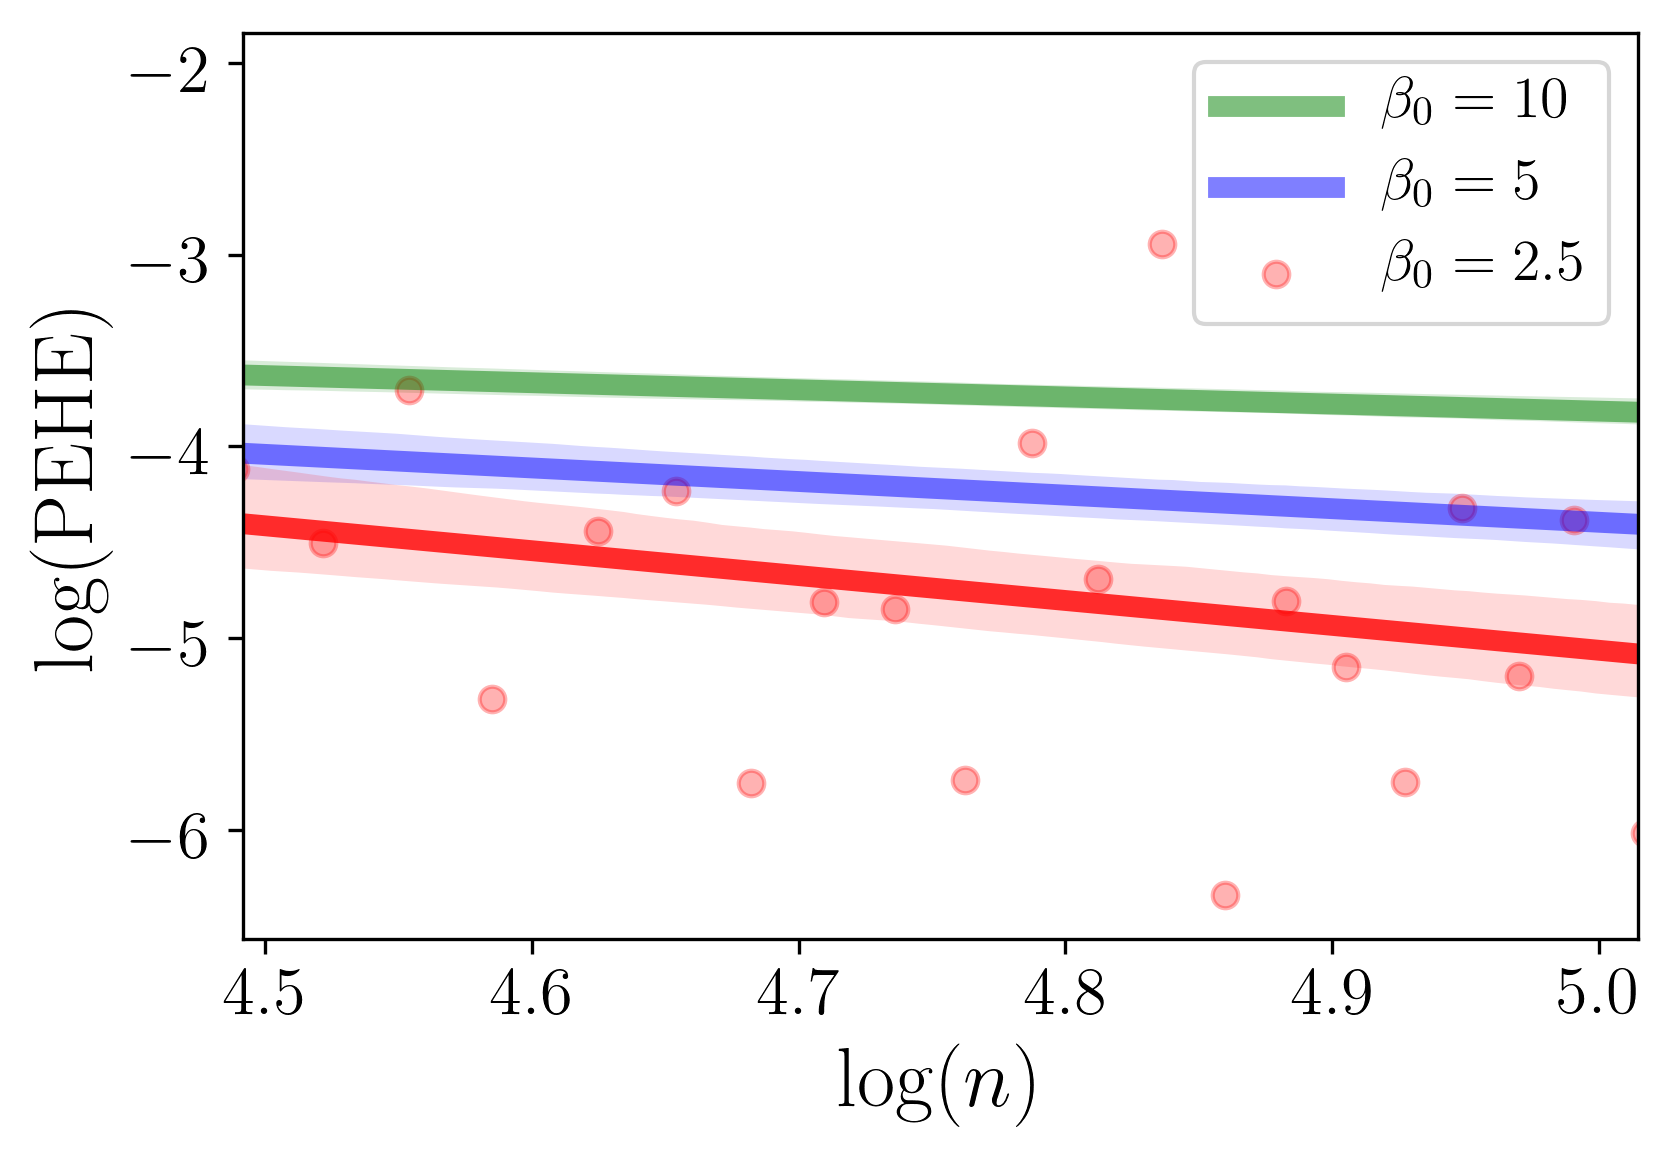
\includegraphics[width=0.9\linewidth]{ch2Fig3.png}
  \caption{\footnotesize Impact of over-smoothed priors.}
  \label{Ahmed2}
\end{subfigure}
\begin{subfigure}{.33\textwidth}
  \centering
  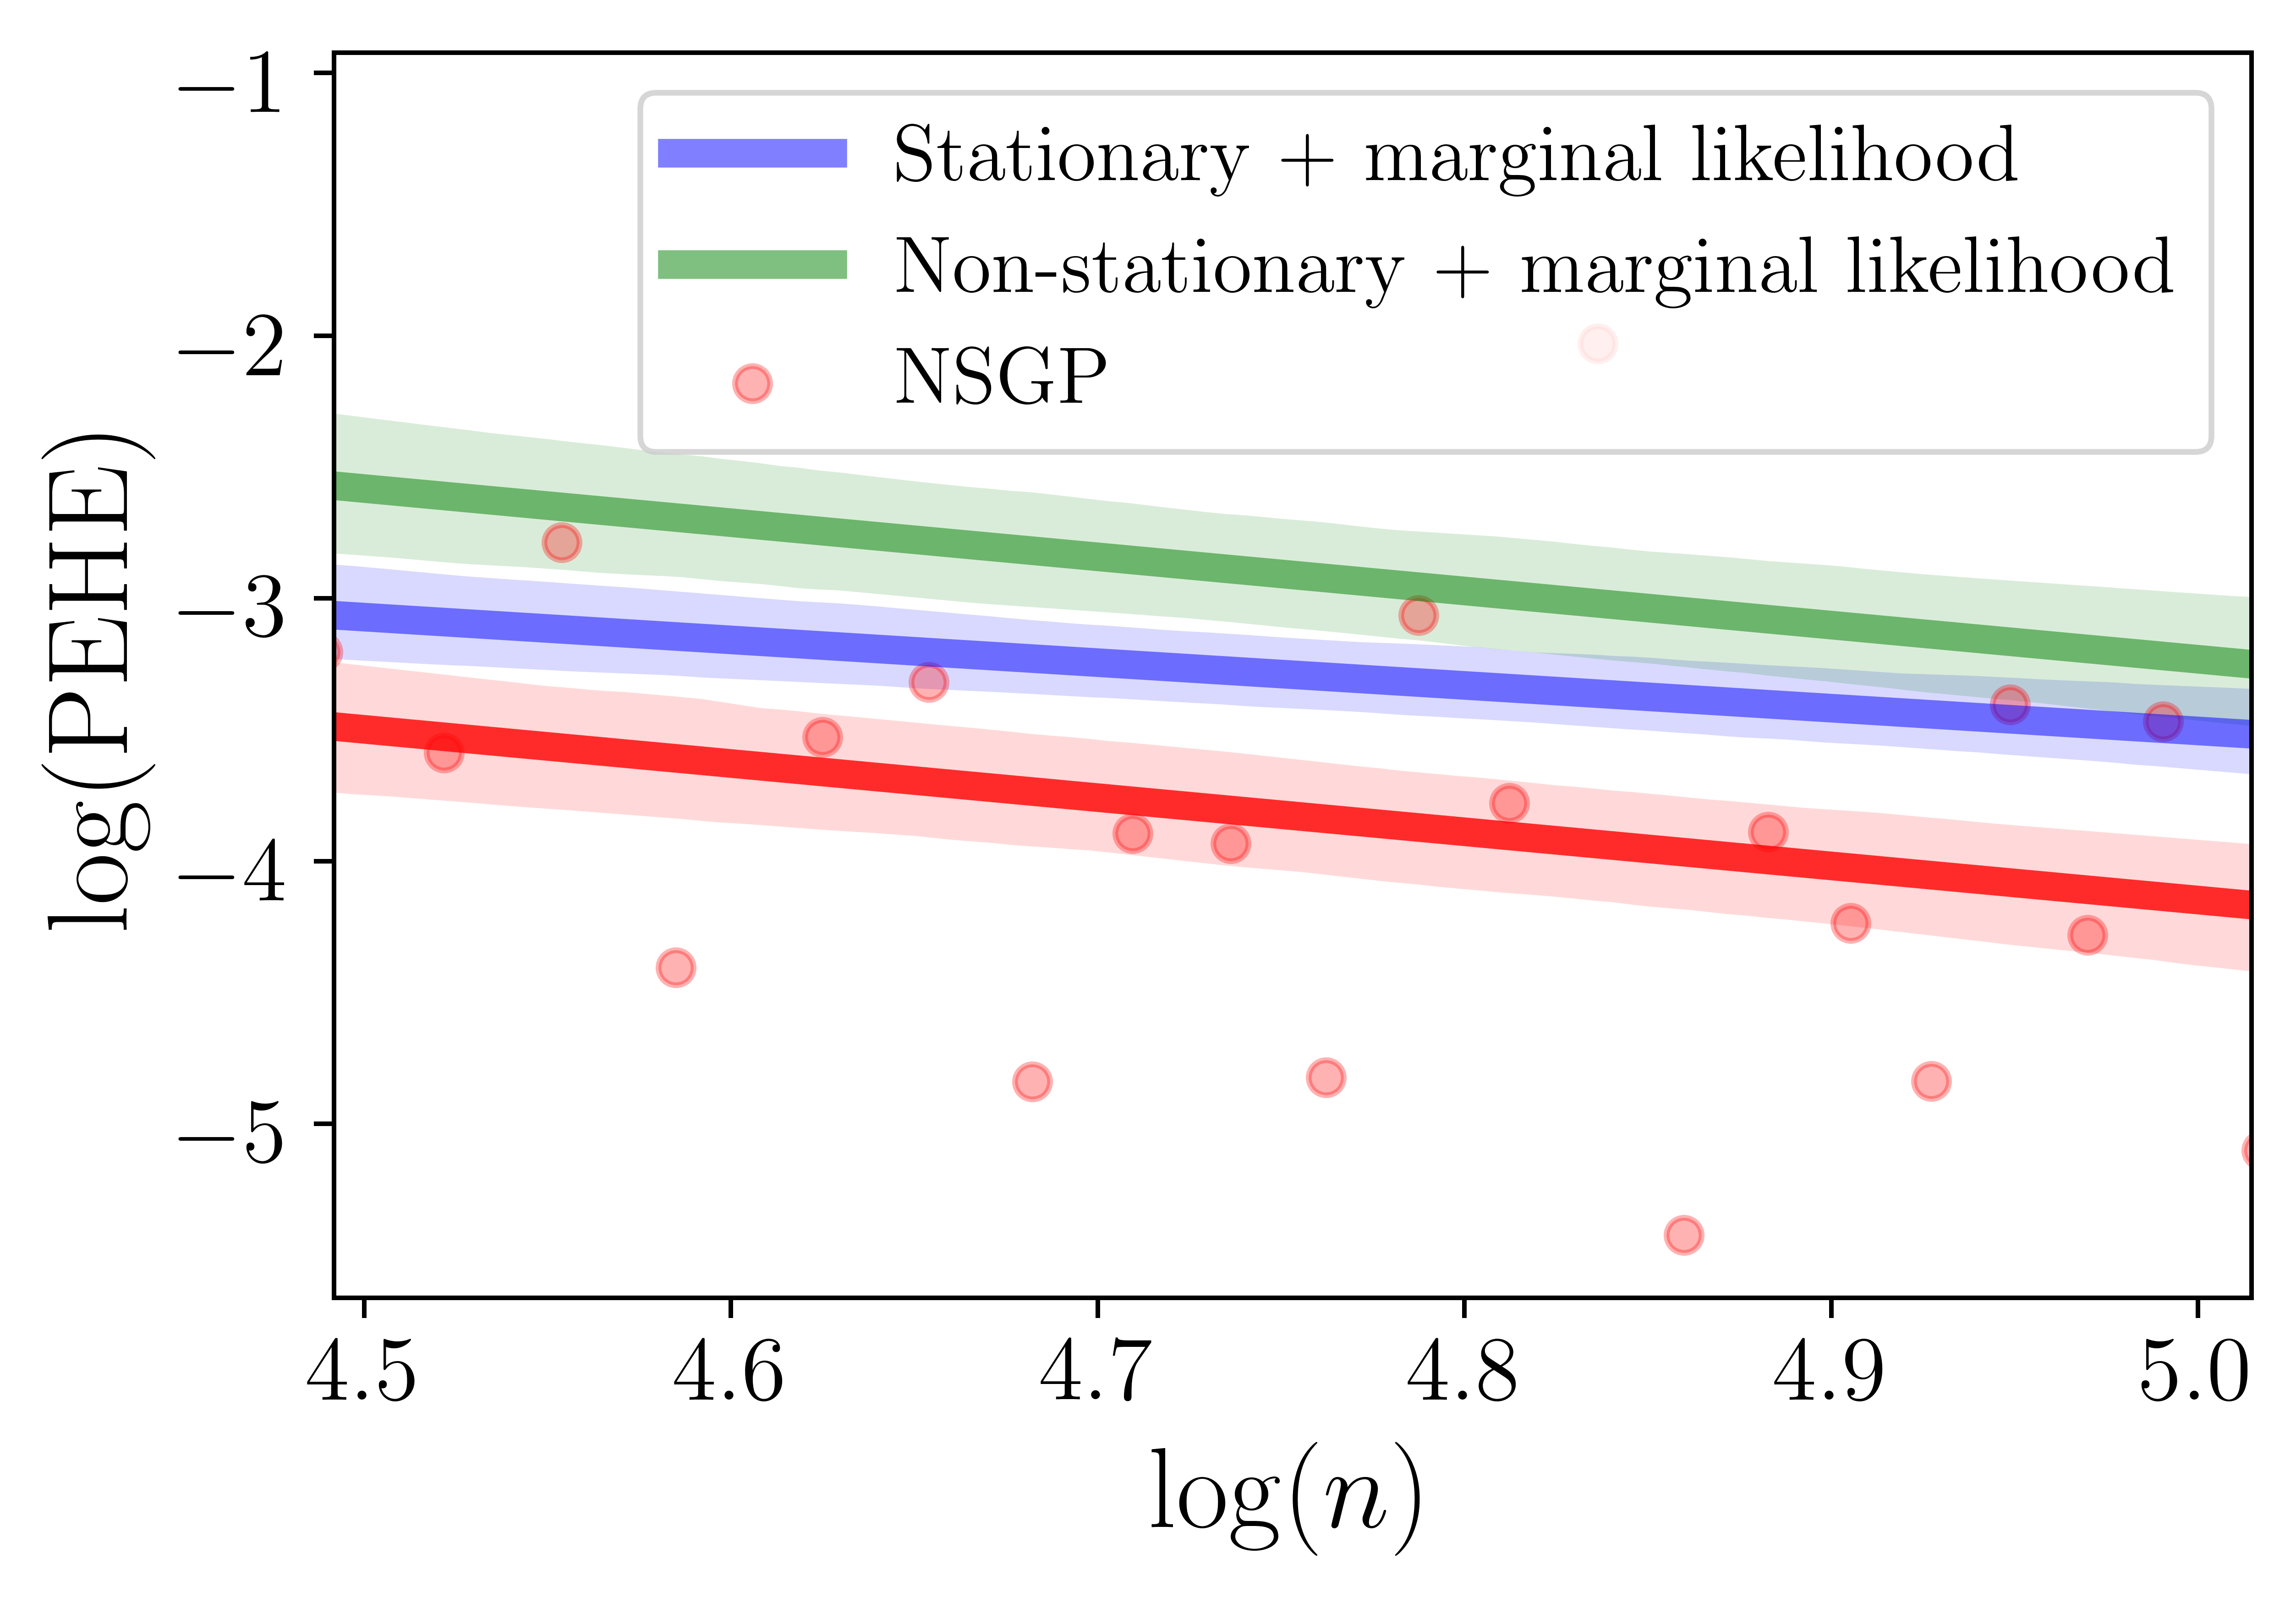
\includegraphics[width=0.9\linewidth]{ch2Fig4.png}
  \caption{\footnotesize Performance of different models.}
  \label{Ahmed3}
\end{subfigure}
	\caption{Scatter-plots and linear fits for the PEHE of NSGP on a $\log$-$\log$ scale in different simulation setups {(RCT: randomized controlled trial)}.}
	\label{ch2Fig2}
\end{figure*}

\section{Experiments}
In this Section, we check the validity of our analyses using a synthetic simulation setup (Subsection \ref{exp1}), and then evaluate the performance of our proposed model using data from a real-world clinical trial with simulated potential outcomes (Subsection \ref{exp2}). We will use the acronym \textbf{NSGP} to refer to the non-stationary GP model proposed in Section \ref{ch2sec4}.  
\subsection{Learning Brownian Response Surfaces}
\label{exp1}
\subsubsection{Synthetic Model}
\label{expexp0}
Let $\mathcal{X} = [0,1]$, and define a $\kappa$-fold integrated Brownian motion $B_{\kappa}$, $\kappa \in \mathbb{N}_+$, on $\mathcal{X}$ as follows:
\begin{align} 
B_{\kappa}(x) = \int_{0}^{x}\int_{0}^{x_\kappa} \cdots \int_{0}^{x_2} B_0(x_1) \,dx_1\, dx_2 \cdots dx_{x_\kappa}, \nonumber 
\end{align}
where $B_0(.)$ is a standard Brownian motion (Wiener process). Sample paths of $B_0$ are almost surely H\"older regular with exponent $\frac{1}{2}$ \cite{karatzas2012brownian}. Since $B_0(x)$ is almost surely non-differentiable everywhere in $\mathcal{X}$, then sample paths of $B_{\kappa}(x)$ are H\"older with exponent $\kappa + \frac{1}{2}$, i.e. $B_{\kappa} \in H^{\kappa+\frac{1}{2}}$ with probability 1. Therefore, when the true response surfaces are $\kappa$-fold integrated Brownian paths, the optimality and achievability results in Theorems 1 and 2 should hold. To this end, we simulate the true response surfaces $f_0 \in H^{\alpha_0}$ and $f_1 \in H^{\alpha_1}$ as $\boldsymbol{f_0 \sim B_{\alpha_0-\frac{1}{2}}}$, and $\boldsymbol{f_1 \sim B_{\alpha_1-\frac{1}{2}}}$, where we set $\boldsymbol{\alpha_0 = 2.5}$ and $\boldsymbol{\alpha_1 = 5.5}$. The propensity score is modeled as a parametrized logistic function $\boldsymbol{p(x\,|\,\eta) = (1+e^{-\eta\,(x-\frac{1}{2})})^{-1}}$, where $\eta \in \mathbb{R}$ is a parameter that determines the severity of selection bias. For a pair of fixed Brownian paths $f_0$ and $f_1$, synthetic observational samples $\boldsymbol{(X_i,W_i,Y^{\mbox{\tiny $(W_i)$}}_i)_i}$ are generated as follows: $\boldsymbol{X_i \sim \mbox{Uniform}[0,1]}$, $\boldsymbol{W_i \sim \mbox{Bernoulli}(p(x\,|\,\eta))}$, and $\boldsymbol{Y^{\mbox{\tiny $(W_i)$}}_i \sim f_{\mbox{\tiny $W_i$}} + \mathcal{N}(0,\sigma^2)}$, where $\boldsymbol{\sigma^2 = 0.1}$. 

\begin{table*}[t]
\centering
%\begin{tcolorbox}[tab3,tabularx={cc|l||c|c|cc|l||c|c}] 
\begin{tabular}{|cc|l||c|c|cc|l||c|c|}
\hline
\textbf{\tiny [Q1]} & \textbf{\tiny [Q2]} & \textbf{\tiny Model} & \textbf{\tiny In-sample $\sqrt{\mbox{PEHE}}$} & \textbf{\tiny Out-of-sample $\sqrt{\mbox{PEHE}}$} & \textbf{\tiny [Q1]} & \textbf{\tiny [Q2]} & \textbf{\tiny Model} & \textbf{\tiny In-sample $\sqrt{\mbox{PEHE}}$} & \textbf{\tiny Out-of-sample $\sqrt{\mbox{PEHE}}$} \\ \hline \hline
\mbox{\footnotesize $\boldsymbol{\checkmark}$} & \mbox{\footnotesize $\boldsymbol{\checkmark}$} & \mbox{\tiny \textbf{NSGP}} & \mbox{\tiny 0.51 $\pm$ 0.013} & \mbox{\tiny 0.64 $\pm$ 0.030} & \mbox{\footnotesize $\boldsymbol{\checkmark}$} & & \mbox{\tiny T-XGBoost} & \mbox{\tiny 1.46 $\pm$ 0.081} & \mbox{\tiny 1.98 $\pm$ 0.152} \\
& & \mbox{\tiny SGP} & \mbox{\tiny 0.95 $\pm$ 0.021} & \mbox{\tiny 1.21 $\pm$ 0.052} & & & \mbox{\tiny S-XGBoost} & \mbox{\tiny 2.97 $\pm$ 0.211} & \mbox{\tiny 3.04 $\pm$ 0.216} \\
\mbox{\footnotesize $\boldsymbol{\checkmark}$} & \mbox{\footnotesize $\boldsymbol{\checkmark}$} & \mbox{\tiny CMGP} & \mbox{\tiny 0.61 $\pm$ 0.011} & \mbox{\tiny 0.76 $\pm$ 0.012} & \mbox{\footnotesize $\boldsymbol{\checkmark}$} & & \mbox{\tiny T-AdaBoost} & \mbox{\tiny 2.40 $\pm$ 0.177} & \mbox{\tiny 2.79 $\pm$ 0.212} \\
\mbox{\footnotesize $\boldsymbol{\checkmark}$} & & \mbox{\tiny TARNet} & \mbox{\tiny 0.88 $\pm$ 0.021} & \mbox{\tiny 0.95 $\pm$ 0.025} & & & \mbox{\tiny S-AdaBoost} & \mbox{\tiny 4.53 $\pm$ 0.317} & \mbox{\tiny 4.56 $\pm$ 0.312} \\
 & \mbox{\footnotesize $\boldsymbol{\checkmark}$} & \mbox{\tiny BNN} & \mbox{\tiny 2.21 $\pm$ 0.115} & \mbox{\tiny 2.15 $\pm$ 0.125} & \mbox{\footnotesize $\boldsymbol{\checkmark}$} & & \mbox{\tiny T-OLS} & \mbox{\tiny 1.85 $\pm$ 0.107} & \mbox{\tiny 1.94 $\pm$ 0.122} \\
\mbox{\footnotesize $\boldsymbol{\checkmark}$} & \mbox{\footnotesize $\boldsymbol{\checkmark}$} & \mbox{\tiny CFR Wass.} & \mbox{\tiny 0.71 $\pm$ 0.018} & \mbox{\tiny 0.76 $\pm$ 0.032} & & & \mbox{\tiny S-OLS} & \mbox{\tiny 5.06 $\pm$ 0.357} & \mbox{\tiny 5.05 $\pm$ 0.352} \\
\mbox{\footnotesize $\boldsymbol{\checkmark}$} & \mbox{\footnotesize $\boldsymbol{\checkmark}$} & \mbox{\tiny CFR MMD} & \mbox{\tiny 0.73 $\pm$ 0.021} & \mbox{\tiny 0.78 $\pm$ 0.022} & \mbox{\footnotesize $\boldsymbol{\checkmark}$} & & \mbox{\tiny T-DNN} & \mbox{\tiny 3.36 $\pm$ 0.137} & \mbox{\tiny 3.46 $\pm$ 0.142} \\
\mbox{\footnotesize $\boldsymbol{\checkmark}$} & & \mbox{\tiny T-Random Forest} & \mbox{\tiny 1.41 $\pm$ 0.071} & \mbox{\tiny 2.21 $\pm$ 0.162} & & & \mbox{\tiny S-DNN} & \mbox{\tiny 3.56 $\pm$ 0.217} & \mbox{\tiny 3.64 $\pm$ 0.212} \\
& & \mbox{\tiny S-Random Forest} & \mbox{\tiny 2.72 $\pm$ 0.241} & \mbox{\tiny 2.91 $\pm$ 0.252} & & \mbox{\footnotesize $\boldsymbol{\checkmark}$} & \mbox{\tiny MARS} & \mbox{\tiny 1.66 $\pm$ 0.106} & \mbox{\tiny 1.74 $\pm$ 0.112} \\
 & \mbox{\footnotesize $\checkmark$} & \mbox{\tiny Causal Forest} & \mbox{\tiny 2.41 $\pm$ 0.141} & \mbox{\tiny 2.82 $\pm$ 0.181} & & & \mbox{\tiny $k$-NN} & \mbox{\tiny 2.69 $\pm$ 0.177} & \mbox{\tiny 4.06 $\pm$ 0.212} \\
& & \mbox{\tiny BART} & \mbox{\tiny 2.00 $\pm$ 0.141} & \mbox{\tiny 2.22 $\pm$ 0.151} & & \mbox{\footnotesize $\boldsymbol{\checkmark}$} & \mbox{\tiny PSM} & \mbox{\tiny 4.92 $\pm$ 0.312} & \mbox{\tiny 4.92 $\pm$ 0.312} \\
& \mbox{\footnotesize $\boldsymbol{\checkmark}$} & \mbox{\tiny BCF} & \mbox{\tiny 1.31 $\pm$ 0.061} & \mbox{\tiny 1.71 $\pm$ 0.102} & & \mbox{\footnotesize $\boldsymbol{\checkmark}$} & \mbox{\tiny TMLE} & \mbox{\tiny 5.27 $\pm$ 0.357} & \mbox{\tiny 5.27 $\pm$ 0.352} \\
\hline
%\end{tcolorbox}
\end{tabular}
\caption{Simulation results for the IHDP dataset. The values reported correspond to the average PEHE (\mbox{\footnotesize $\pm$ 95$\%$ confidence intervals}).}
\label{TableCh1}
\end{table*}


\subsubsection{Experiments and Results}  
\label{expexp}
Using the setup in Section \ref{expexp0}, we conducted the following Monte Carlo simulations to verify our theoretical findings and highlight the merits of our NSGP model. 	

\textbf{$\bullet$ \textit{Verifying Theorems 1 and 2}:} In order to check the validity of the results of Theorems 1 and 2, we use a NSGP Mat\'ern prior $\mathcal{GP}(0,\boldsymbol{K}_{\beta})$, with length-scale parameters $\beta_0$ and $\beta_1$ that are matched exactly with the regularities of the Brownian paths $f_0$ and $f_1$ (i.e., $\beta_0 = 2.5$ and $\beta_1 = 5.5$). According to Theorem 1, the optimal rate for estimating the CATE $T = f_1 - f_0$ is $n^{\frac{-5}{6}}$, and from Theorem 2, the NSGP with $\beta_0 = 2.5$ and $\beta_1 = 5.5$ should achieve that rate. 

Figure \ref{ch2Fig2} provides a scatter-plot for the PEHE achieved by the NSGP with respect to the number of samples on a $\log$-$\log$ scale for different settings of $\eta$. We fit a linear regression model that describes the PEHE behavior in the $\log$-$\log$ scale. We found the slope of the linear fit to be 0.8437, which is very close\footnote{The minor discrepancy is a result of the residual error in the linear regression fit.} to the slope of $\frac{5}{6} \approx 0.833$ predicted by Theorem 1. Moreover, by changing the magnitude of $\eta$ from $0$ to $\frac{1}{2}$, the PEHE curve did not exhibit any significant change in its slope, and was only moved upwards by a constant offset. On the contrary, Figure \ref{ch2Fig2} shows the PEHE behavior when the NSGP prior is over-smoothed ($\beta_0 > \alpha_0$) for $\eta=0$: as predicted by Theorem 2, learning becomes sluggish (slopes become less steep) as $\beta_0$ increase since the matching condition in (\ref{ch2eq11}) does not hold any more.     

\textbf{$\bullet$ \textit{NSGPs do not leave any money on the table:}} In this experiment, we show that the different components of the NSGP model allow it to perform well in small and large sample regimes. We set a strong selection bias of $\eta = \frac{1}{2}$ and compare the $\log(\mbox{PEHE})$ characteristic of NSGP with a model that uses the same non-stationary kernel as NSGP, and another model that uses a standard stationary kernel, but both models are tuned using marginal likelihood maximization. As we can see in Figure \ref{ch2Fig2}, the model with the non-stationary kernel achieves the same learning rate as NSGP, but exhibits a large offset as it does not account for selection bias, whereas the stationary model fails to learn the smoothness of the rougher Brownian motion since it assigns the same length-scale to both surfaces, and hence it over-smooths the prior, achieving a suboptimal rate. 

\subsection{The Infant Health and Development Program}
\label{exp2}
We evaluated the performance of the NSGP model presented in Section \ref{ch2sec41} using the standard semi-synthetic experimental setup designed by Hill in \cite{hill2011bayesian}. We report a state-of-the-art result in this setup, and draw connections between our experimental results and our analyses.

\subsubsection{Data and Benchmarks}
\label{expexp0ZXC}  
The Infant Health and Development Program (IHDP) is an interventional program intended to enhance the health of premature infants \cite{hill2011bayesian}. \cite{hill2011bayesian} extracted features and treatment assignments from a real-world clinical trial, and introduced selection bias to the data artificially by removing a subset of the patients. The potential outcomes are simulated according to the standard non-linear "Response Surface B" setting in \cite{hill2011bayesian}. The dataset comprised 747 subjects, with 25 features for each subject. Our experimental setup is identical to \cite{hill2011bayesian,johansson2016learning,shalit2016estimating,alaa2017bayesian}: we run 1000 experiments in which we compute the in-sample and out-of-sample $\sqrt{\mbox{PEHE}}$ (with 80/20 training/testing splits), and report average results in Table \ref{TableCh1}. 

We compared the performance of NSGP with a total of 23 CATE estimation benchmarks. We considered: tree-based algorithms (BART \cite{hill2011bayesian}, Causal forests \cite{wager2017estimation}, Bayesian causal forests \cite{hahn2017bayesian}), methods based on deep learning (CFR Wass., CFR MMD, BNN, TARnet \cite{shalit2016estimating}), multivariate additive regression splines (MARS) \cite{powers2017some}, Gaussian processes (CMGP) \cite{alaa2017bayesian}, nearest neighbor matching ($k$-NN), propensity score matching (PSM), and targeted maximum likelihood (TMLE) \cite{porter2011relative}. We also composed a number of T-learners and S-learners as in \cite{kunzel2017meta}, using a variety of baseline machine learning algorithms (DNN stands for deep networks and OLS stands for linear regression). 

\subsubsection{Results and Conclusions}  
\label{expexpZZZ}
As we can see in Table \ref{TableCh1}, the proposed NSGP model significantly outperforms \textbf{all} competing benchmarks. The combined benefit of the two components of an NSGP (non-stationary kernel and doubly-robust hyperparameters) is highlighted by comparing its performance to a vanilla SGP (stationary GP) with marginal likelihood maximization. The gain with respect to such a model is a 2-fold improvement in the PEHE. 

Because the IHDP dataset has a ``moderate" sample size, both selection bias and learning rate seem to impact the performance. Thus, our method took advantage of having addressed modeling questions \textbf{[Q1]} and \textbf{[Q2]} appropriately by being both ``rate-optimal" and ``bias-aware". 

The check marks in columns \textbf{[Q1]} and \textbf{[Q2]} designate methods that address modeling questions \textbf{[Q1]} and \textbf{[Q2]} ``appropriately" in the light of the analysis presented in Section \ref{ch2sec3}. Methods with \textbf{[Q1]} checked use a regression structure with ``outcome-specific" hyperparameters, and methods with \textbf{[Q2]} checked adjust for selection bias. A general observation is that the structure of the regression model seem to matter much more than the strategy for handling selection bias. This is evident from the fact that the TARnet model (does not handle bias but models outcomes separately) significantly outperforms BNN (handles bias but uses a single-surface model \cite{shalit2016estimating}), and that all T-learners (models 2 separate response surfaces) outperformed their S-shaped counterparts (models a single surface). For parametric models, such as OLS, the issue of selecting the right regression structure is even more crucial. 

To sum up, the results in Table \ref{TableCh1} imply that selecting the right regression structure is crucial for rate-optimality in sufficiently large dataset, whereas handling selection bias provides an extra bonus. In Table \ref{TableCh1}, methods that address both \textbf{[Q1]} and \textbf{[Q2]} (NSGP, CMGP, and CFR. Wass and MMD) displayed a superior performance.

\chapter{Symbolic Approaches to Prognostic Model Interpretability}

The ability to interpret the predictions of a (predictive or causal) machine learning model brings about patient and clinician trust, and supports understanding of the underlying disease being modeled \cite{lundberg2017unified,lipton2016mythos, alaa2019}. In many clinical settings, interpretability can be a crucial requirement for the deployment of machine learning, since a model's predictions would inform critical decision-making. Model explanations can also be central in other domains, such as natural sciences \cite{schmidt2009distilling,wang2019symbolic}, where the primary utility of a model is to help understand an underlying phenomenon, rather than merely making predictions about it. Unfortunately, most state-of-the-art models --- such as ensemble~models, kernel methods, and neural networks --- are perceived as being complex ``black-boxes'', the predictions of which are too hard to be interpreted by human subjects \cite{lundberg2017unified,yoon2018invase,jordon2018knockoffgan,shrikumar2017learning,lou2013accurate,elenberg2017streaming,bouchard2017union,melis2018towards,tsang2018neural,zhang2018interpreting,chen2018learning,ribeiro2016should}. 

\begin{figure*}[t]
\centering
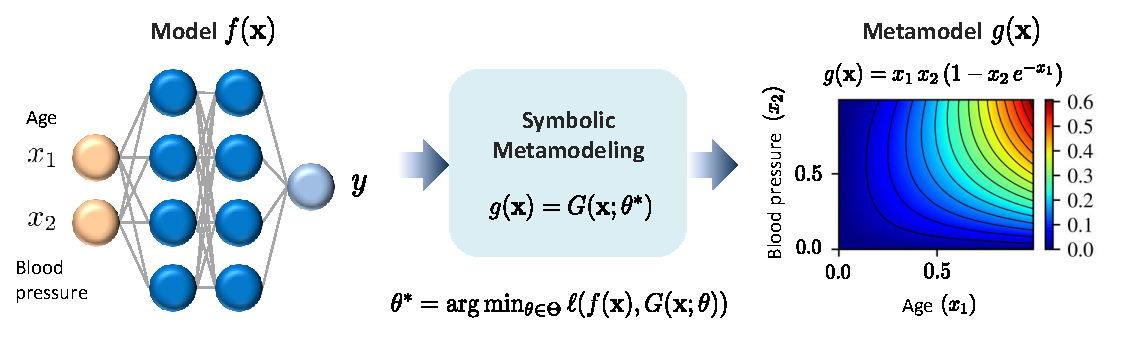
\includegraphics[width=6in]{ch3Fig1.pdf}
\caption{Pictorial depiction of the symbolic metamodeling framework. Here, the model $f(\boldsymbol{x})$ is a deep neural network (left), and the metamodel $g(\boldsymbol{x})$ is a closed-form expression $x_1\,x_2\,(1-x_2\,\exp(-x_1))$ (right).}
\label{ch3fig1} 
\end{figure*}

In this Chapter, we approach the problem of model interpretation by introducing the \textit{symbolic metamodeling} framework for expressing black-box models in terms of transparent mathematical equations that can be easily understood and analyzed by human subjects (Section \ref{ch3sec2}). The proposed metamodeling procedure takes as an input a (trained) model --- represented by a black-box function $f(\boldsymbol{x})$ that maps a feature $\boldsymbol{x}$ to a prediction $y$ --- and retrieves a \textit{symbolic metamodel} $g(\boldsymbol{x})$, which is meant to be an interpretable mathematical abstraction of $f(\boldsymbol{x})$. The metamodel $g(\boldsymbol{x})$ is a tractable symbolic expression comprising a finite number of familiar functions (e.g., polynomial, analytic, algebraic, or closed-form expressions) that are combined via elementary arithmetic operations (i.e., addition and multiplication), which makes it easily understood by inspection, and can be analytically manipulated via symbolic computation engines such as {\small \texttt{Mathematica}} \cite{abell2017mathematica}, {\small \texttt{Wolfram alpha}} \cite{wolfram2013wolfram}, or {\small \texttt{Sympy}} \cite{10.7717/peerj-cs.103}. Our approach is appropriate for models with small to moderate number of features, where the physical interpretation of these features are of primary interest. 

A high-level illustration of the proposed metamodeling approach is shown in Figure \ref{ch3fig1}. In this Figure, we consider an example of using a neural network to predict the risk of cardiovascular disease based on a (normalized) feature vector ${\bf x} = (x_1, x_2)$, where $x_1$ is a person's age and $x_2$ is their blood pressure. For a clinician using this model in their daily practice or in the context of an epidemiological study, the model $f({\bf x})$ is completely obscure --- it is hard to explain or draw insights into the model's predictions, even with a background knowledge of neural networks. On the other hand, the metamodel $g({\bf x}) = x_1\,x_2\,(1-x_2\exp(-x_1))$ is a fully transparent abstraction of the neural network model, from which one can derive explanations for the model's predictions through simple analytic manipulation, without the need to know anything about the model structure and its inner workings\footnote{Note that here we are concerned with explaining the predictions of a trained model, i.e., its \textit{response surface}. Other works, such as \cite{koh2017understanding}, focus on explaining the model's \textit{loss surface} in order to understand how it learns.}. Having such an explicit (simulatable) equation for predicting risks is already required by various clinical guidelines to ensure the transparency of prognostic models \cite{kattan2016american}. 

In order to find the symbolic metamodel $g({\bf x})$ that best approximates the original model $f({\bf x})$, we need to search a space of mathematical expressions and find the expression that minimizes a ``metamodeling loss'' $\ell(g({\bf x}), f({\bf x}))$. But how can we construct a space of symbolic expressions without predetermining its functional from? In other words, how do we know that the metamodel $g({\bf x}) = x_1\,x_2\,(1-x_2\exp(-x_1))$ in Figure \ref{ch3fig1} takes on an exponential form and not, say, a trigonometric or a polynomial functional form?   

To answer this question, we introduce a novel parameterized representation of symbolic expressions (Section \ref{ch3sec3}), $G({\bf x};\theta)$, which reduces to most familiar functional forms --- e.g., arithmetic, polynomial, algebraic, closed-form, and	analytic expressions, in addition to special functions, such as Bessel functions and Hypergeometric functions --- for different settings of a real-valued parameter $\theta$. The representation $G({\bf x};\theta)$ is based on Meijer $G$-functions \cite{meijer1946gfunc,meijer1936uber,beals2013meijer}, a class of contour integrals used in the mathematics community to find closed-form solutions for otherwise intractable integrals. The proposed Meijer $G$-function parameterization enables minimizing the metamodeling loss efficiently via gradient descent --- this is a major departure from existing approaches to {\it symbolic regression}, which use genetic programming to select among symbolic expressions that comprise a small number of predetermined functional forms \cite{orzechowski2018we,menezes2014symbolic,vladislavleva2009order}. 

Existing methods for model interpretation focus on crafting explanation models that support only one ``mode'' of model interpretation. For instance, methods such as DeepLIFT \cite{shrikumar2017learning} and LIME \cite{ribeiro2016should}, can explain the predictions of a model in terms of the contributions of individual features to the prediction, but cannot tell us whether the model is nonlinear, or whether statistical interactions between features exist. Other methods such as GA$^2$M \cite{lou2013accurate} and NIT \cite{tsang2018neural}, focus exclusively on uncovering the statistical interactions captured by the model, which may not be the most relevant mode of explanation in many application domains. Moreover, none of the existing methods can uncover the functional forms by which a model captures nonlinearities in the data --- such type of interpretation is important in applications such as applied physics and material sciences, since researchers in these fields focus on distilling an analytic law that describes how the model fits experimental data \cite{schmidt2009distilling,wang2019symbolic}.  

Our perspective on model interpretation departs from previous works in that, a symbolic metamodel $g({\bf x})$ is not hardwired to provide any specific type of explanation, but is rather designed to provide a full mathematical description of the original model $f({\bf x})$. In this sense, symbolic metamodeling should be understood as a tabula rasa upon which different forms of explanations can be derived --- as we will show in Section \ref{ch3sec4}, most forms of model explanation covered in previous literature can be arrived at through simple analytic manipulation of a symbolic metamodel. 

\begin{figure*}[t]
\centering
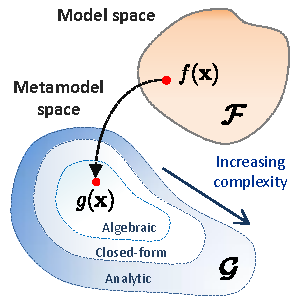
\includegraphics[width=2.5in]{ch3Fig2.pdf}
\caption{The metamodeling problem.}
\label{ch3fig2} 
\end{figure*}

\section{Symbolic Metamodeling}
\label{ch3sec2}
Let $f:\mathcal{X} \to \mathcal{Y}$ be a machine learning model trained to predict a target outcome $y \in \mathcal{Y}$ on the basis of a $d$-dimensional feature instance ${\bf x} = (x_{1},\ldots,x_{d}) \in \mathcal{X}$. We assume that $f(.)$ is a {\it black-box} model to which we only have query access, i.e., we can evaluate the model's output $y = f({\bf x})$ for any given feature instance ${\bf x}$, but we do not know the model's internal structure. Without loss of generality, we assume that the feature space $\mathcal{X}$ is the unit hypercube, i.e., $\mathcal{X} = [0,1]^d$.\\
\\
{\bf The metamodeling problem.} A {\it symbolic metamodel} $g \in \mathcal{G}$ is a ``model of the model'' $f$ that approximates $f({\bf x})$ for all ${\bf x} \in \mathcal{X}$, where $\mathcal{G}$ is a class of succinct mathematical expressions that are understandable to users and can be analytically manipulated. Typically, $\mathcal{G}$ would be set as the class of all arithmetic, polynomial, algebraic, closed-form, or analytic expressions. Choice of $\mathcal{G}$ will depend on the desired complexity of the metamodel. In most medical applications, we might opt to restrict $\mathcal{G}$ to algebraic expressions. Given $\mathcal{G}$, the metamodeling problem consists in finding the function $g$ in $\mathcal{G}$ that bests approximates the model $f$.

Figure \ref{ch3fig2} shows a pictorial depiction of the metamodeling problem as a mapping from the {\it modeling space} $\mathcal{F}$ --- i.e., the function class that the model $f$ inhabits\footnote{For instance, for an $L$-layer neural network, $\mathcal{F}$ is the space of compositions of $L$ nested activation functions. For a random forest with $L$ trees, $\mathcal{F}$ is the space of summations of $L$ piece-wise functions.} --- to the interpretable metamodeling space $\mathcal{G}$. Metamodling is only relevant when $\mathcal{F}$ spans functions that are considered uninterpretable to users. For models that are deemed interpretable, such as linear regression, $\mathcal{F}$ will already coincide with $\mathcal{G}$, because the linear model is already an algebraic expression (and a first-order polynomial). In this case, the best metamodel for $f$ is the model $f$ itself, i.e., $g = f$.

Formally, metamodeling can be formulated through the following optimization problem:  
\begin{align}
g^* = \arg \min_{g \in \mathcal{G}} \ell(g, f),\,\,\,\,\,\, \ell(g, f) = \|\,f\, - \,g\,\|_2^2 = \int_{\mathcal{X}} (g({\bf x}) - f({\bf x}))^2\, d{\bf x},
\label{ch3eq1}
\end{align}
where $\ell(.)$ is the {\it metamodeling loss}, which we set to be the mean squared error (MSE) between $f$ and $g$. In the following Section, we will focus on solving the optimization problem in (\ref{ch3eq1}).

\section{Metamodeling via Meijer $G$-functions}
\label{ch3sec3}
In order to solve the optimization problem in (\ref{ch3eq1}), we need to induce some structure into the metamodeling space $\mathcal{G}$. This is obviously very challenging since $\mathcal{G}$ encompasses infinitely many possible mathematical expressions with very diverse functional forms. For instance, consider the exemplary metamodel in Figure \ref{ch3fig1}, where $g({\bf x}) = x_1\,x_2\,(1-x_2\exp(-x_1))$. If $\mathcal{G}$ is set to be the space of all closed-form expressions, then it would include all polynomial, hyperbolic, trigonometric, logarithmic functions, rational and irrational exponents, and any combination thereof \cite{chow1999closed,borwein2013closed}. Expressions such as $g^{\prime}({\bf x}) = (x^2_1 + x^2_2)$ and $g^{\prime\prime}({\bf x}) = \sin(x_1)\cdot \cos(x_2)$ are both valid metamodels, i.e., $g^{\prime}, g^{\prime\prime} \in \mathcal{G}$, yet they each have functional forms that are very different from $g$. Thus, we need to parameterize $\mathcal{G}$ in such a way that it encodes all such functional forms, and enables an efficient solution to (\ref{ch3eq1}). 

To this end, we envision a parameterized metamodel $g({\bf x}) = G({\bf x};\theta),\, \theta \in \Theta$, where $\Theta = \mathbb{R}^M$ is a parameter space that fully specifies the metamodeling space $\mathcal{G}$, i.e., $\mathcal{G} = \{G(.;\theta): \theta \in \Theta\}$. Such parameterization should let $G({\bf x};\theta)$ reduce to different functions for different settings of $\theta$ --- for the aforementioned example, we should have $G({\bf x};\theta^{\prime}) = (x^2_1 + x^2_2)$ and $G({\bf x};\theta^{\prime\prime}) = \sin(x_1)\cdot \cos(x_2)$ for some $\theta^{\prime}, \theta^{\prime\prime} \in \Theta$. Given the parameterization $G({\bf x};\theta)$, the problem in (\ref{ch3eq1}) reduces to  
\begin{align}
g^*({\bf x}) = G({\bf x};\theta^*),\,\,\mbox{where}\,\, \theta^* = \arg \min_{\theta \in \Theta}\,\, \ell(G({\bf x};\theta), f({\bf x})).
\label{eq0x3}
\end{align}
Thus, if we have a parameterized symbolic expression $G({\bf x};\theta)$, then metamodeling boils down to a straightforward parameter optimization problem. We construct $G({\bf x};\theta)$ in Section \ref{Sec31}.

\subsection{Parameterizing symbolic metamodels with Meijer $G$-functions}
\label{Sec31}
We propose a parameterization of $G({\bf x};\theta)$ that includes two steps. The first step involves decomposing $G({\bf x};\theta)$ into a combination of univariate functions. The second step involves modeling these univariate functions through a very general class of special functions that includes most known familiar functions as particular cases. Both steps are explained in detail in what follows. \\   
\\
{\bf Step 1: Decomposing the metamodel.} We breakdown the {\it multivariate} function $g({\bf x})$ into simpler, {\it univariate} functions. From the {\it Kolmogorov superposition theorem} \cite{kolmogorov1957representation}, we know that every multivariate continuous function $g({\bf x})$ can be written as a finite composition of univariate continuous functions and the addition operation as follows\footnote{The Kolmogorov decomposition in (\ref{ch3eq3}) is a universal function approximator \cite{hornik1989multilayer}. In fact, (\ref{ch3eq3}) can be thought of as a 2-layer neural network with generalized activation functions \cite{kuurkova1992kolmogorov, girosi1989representation, igelnik2003kolmogorov, hornik1989multilayer, cybenko1989approximation}.}:  
\begin{equation}
g(\mathbf{x}) = g(x_{1},\ldots,x_{n}) = \sum_{i=0}^{r}g^{out}_{i}\left(\,\sum_{j=1}^{d}g^{in}_{ij}(x_{j})\,\right),
\label{ch3eq3}
\end{equation}
where $\mbox{\footnotesize $g_i^{in}$}$ and $\mbox{\footnotesize $g_{ij}^{out}$}$ are continuous univariate {\it basis functions}, and $r \in \mathbb{N}_+$. The exact decomposition in (\ref{eq1x}) always exists for $r = 2d$, and for some basis functions $\mbox{\footnotesize $g_i^{out}: \mathbb{R} \to \mathbb{R}$}$, and $\mbox{\footnotesize $g_{ij}^{in}: [0,1] \to \mathbb{R}$}$ \cite{sprecher1993universal}. When $r=1$, (\ref{eq1x}) reduces to the generalized additive model \cite{hastie2017generalized}. While we proceed our analysis with the general formula in (\ref{ch3eq3}), in our practical implementation we set $r=1$, $g^{out}$ as the identify function, and include extra functions $g^{in}_{ij}$ of the interactions $\{x_i\,x_j\}_{i,j}$ to account for the complexity of $g(\mathbf{x})$. 



\section{Experiments}
\label{ch3sec4}

\chapter{Automated Prognostic Modeling}

\chapter{Deep Probabilistic Modeling of Longitudinal Data}

For text, let's use the first words out of the ispell dictionary.

\chapter{Clinical Application}

\chapter{Conclusions}

\bibliographystyle {unsrt} %{thesis}
\bibliography {thesisrefs}    % bibliography references

\end {document}

